\documentclass[[12pt,oneside,openany,a4paper, %... Layout
english, %... Global lang drivers{}
masters-t, goldenblock]{usthesis} 
\usepackage{graphicx}
\usepackage[colorinlistoftodos,prependcaption,textsize=small,disable]{todonotes}
\usepackage{pgfgantt}
\usepackage{float} %so that it can use the 'f' float option
\usepackage{pdflscape} %allow you to make landscape pages
\usepackage{amsmath}
\newcommand*\mean[1]{\bar{#1}} % to create an overbar for symbols
% \usepackage{cite}
\usepackage{soul}
\usepackage{amssymb}
\usepackage{bm}
\usepackage{standalone}
\usepackage{preview}
\usepackage{mathtools}
\usepackage{pdfpages}
% \usepackage[sort&compress]{natbib} %able to cite 2 reference at once
\usepackage{cite}
% \usepackage{gensymb} %for degree symbol
% \usepackage{hyperref} %to hyperlink the equations

\newganttlinktype{drur}{
\ganttsetstartanchor{on bottom=0.75}
\ganttsetendanchor{on left}
\draw [/pgfgantt/link]
% first segment (down)
(\xLeft, \yUpper) --
% second segment (right)
(\xLeft, \yUpper -
\ganttvalueof{link bulge} * \ganttvalueof{y unit chart}) --
% link label
node [pos=.5, /pgfgantt/link label anchor] {\ganttlinklabel}
% third segment (up)
($(\xLeft,
\yUpper -
\ganttvalueof{link bulge} * \ganttvalueof{y unit chart})!%
\ganttvalueof{link mid}!%
(\xRight,
\yUpper -
\ganttvalueof{link bulge} * \ganttvalueof{y unit chart})$) --
% last segment (right again)
($(\xLeft, \yLower)!%
\ganttvalueof{link mid}!%
(\xRight, \yLower)$) --
(\xRight, \yLower);
}

\newganttlinktype{rdldr*}{%
  \draw [/pgfgantt/link]
    (\xLeft, \yUpper) --
    (\xLeft + \ganttvalueof{link bulge 1} * \ganttvalueof{x unit},
      \yUpper) --
    ($(\xLeft + \ganttvalueof{link bulge 1} * \ganttvalueof{x unit},
      \yUpper)!%
      \ganttvalueof{link mid}!%
      (\xLeft + \ganttvalueof{link bulge 1} * \ganttvalueof{x unit},
      \yLower)$) --
    ($(\xRight - \ganttvalueof{link bulge 2} * \ganttvalueof{x unit},
      \yUpper)!%
      \ganttvalueof{link mid}!%
      (\xRight - \ganttvalueof{link bulge 2} * \ganttvalueof{x unit},
      \yLower)$) --
    (\xRight - \ganttvalueof{link bulge 2} * \ganttvalueof{x unit},
      \yLower) --
    (\xRight, \yLower);%
}
\ganttset{
  link bulge 1/.link=/pgfgantt/link bulge,
  link bulge 2/.link=/pgfgantt/link bulge}

\begin{document}

\includepdf{Cover.pdf}
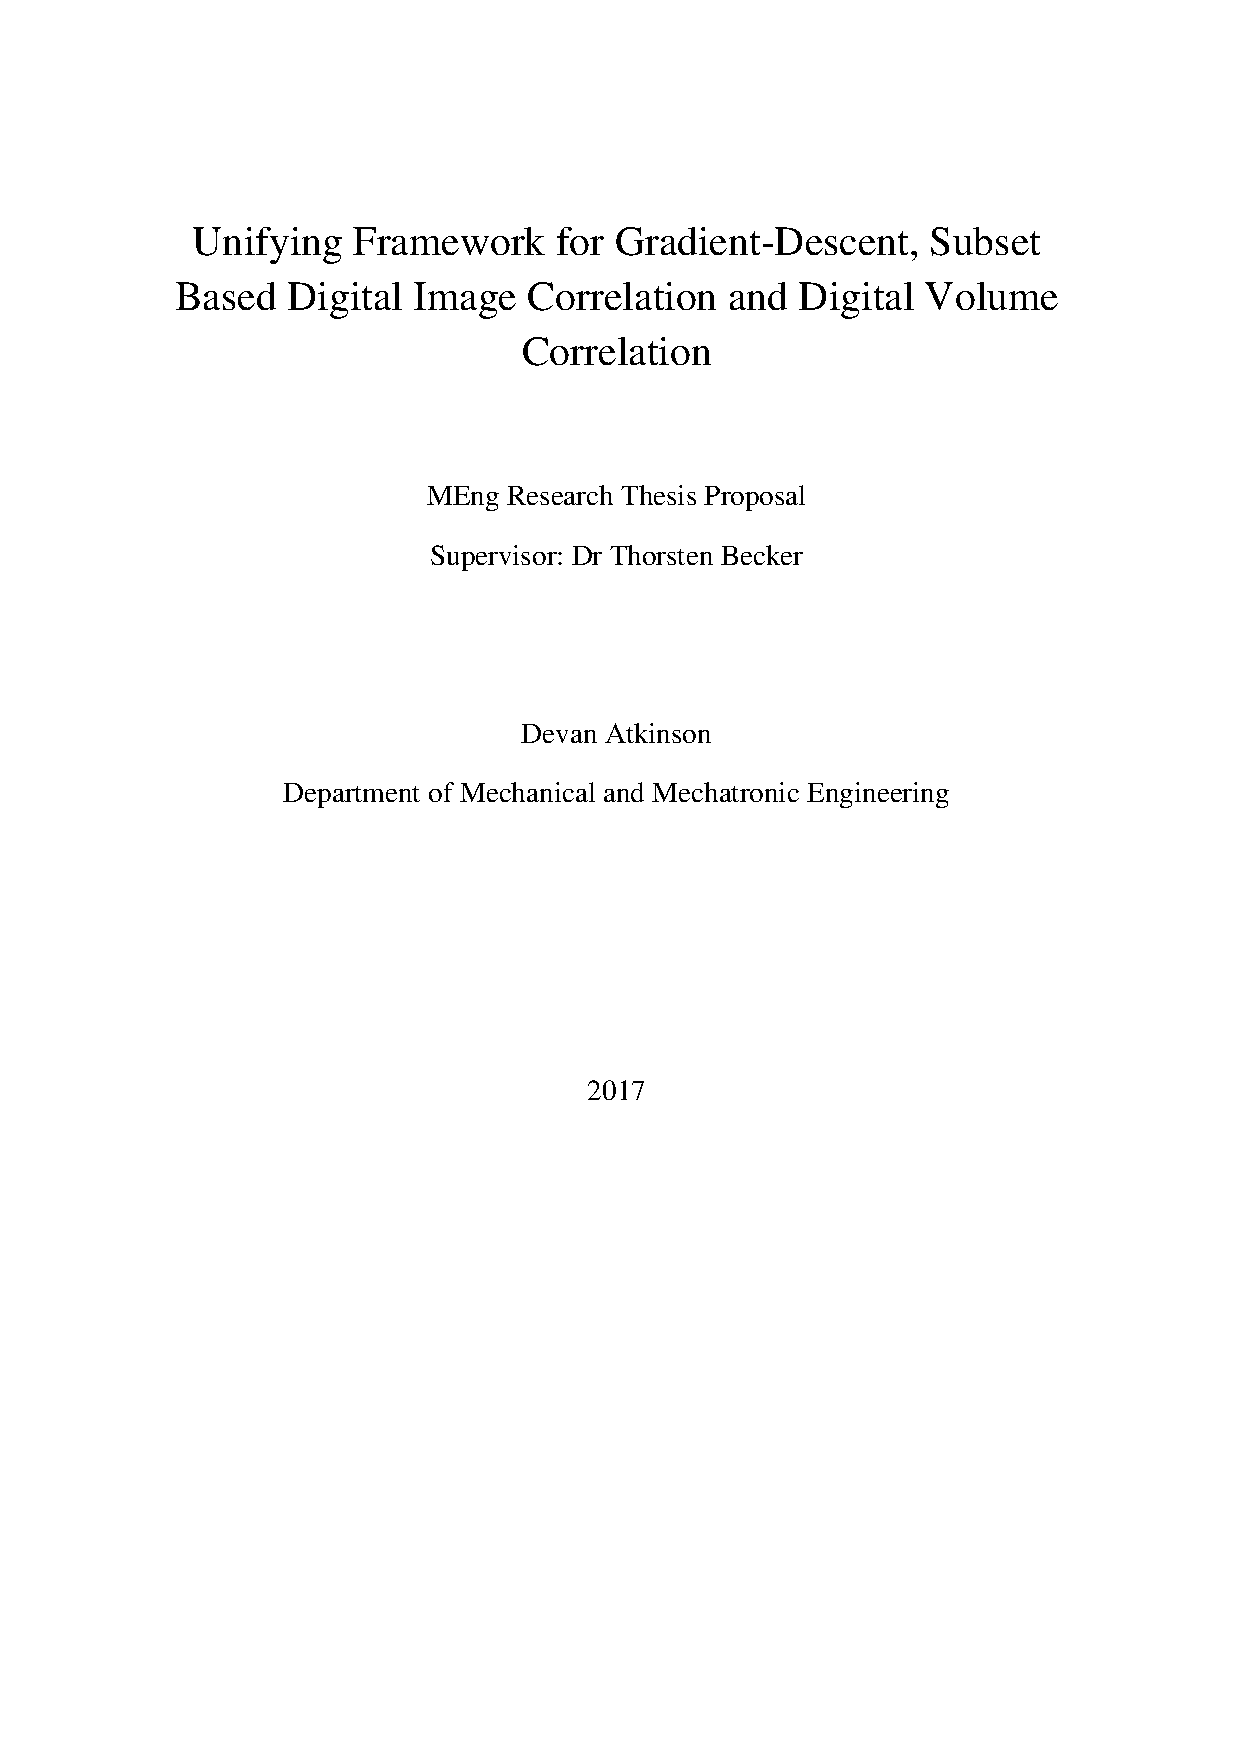
\includepdf{TitlePage.pdf}

\includepdf{plagiarism.pdf}
\chapter*{Abstract}
Digital Image Correlation (DIC) and Digital Volume Correlation (DVC) are becoming widely used tools, in the field of material science, to measure the displacements and deformations of specimens. However the high cost of commercial DIC and DVC software and the limited control offered over the correlation process in both commercial and open-source software limits its widespread adoption. This paper proposes a project which aims to create a Matlab based program capable of performing 2D DIC and DVC on a given set of images while allowing the user control over the correlation process. It is hypothesised that the different DIC algorithms use different methods to perform the same tasks in the correlation process. Thus by analysing these algorithms it is possible to combine these different methods into one program which will allow the user to select which methods to use for the various correlation tasks. If successful, this project will produce a freely available program, which offers many of the correlation methods of the different DIC algorithms, so that users will be able to perform in depth DIC and DVC analyses.

% which allows users full control over the correlation process 

% This project primarily consists of researching different DIC algorithms to determine the various methods of performing correlation and incorporating these methods into the program so that the user can choose which to use.



%  This project is motivated by the lack of freely available DIC software which allows the user to control the correlation process. This software is intended to combine most of the 2D DIC algorithms that are beneficial to material science applications into a single code. The successful completion of this project  will allow researchers of material science a comprehensive tool to determine specimen deformation from images taken of the specimen.

\tableofcontents
\listoffigures
\chapter{Introduction}
\section{Background}
Digital Image Correlation (DIC) and Digital Volume Correlation (DVC) fall into the discipline of computer vision which aims to extract quantifiable information from images. This quantifiable information that DIC extracts is the optical flow that occurs between two images. It is capable of relating this optical flow to the displacements and deformations of the physical objects captured in the images. Thus it constitutes a tool for determining the displacements and deformations of 3D objects from images taken of these objects. Since its introduction its has found widespread use in many applications including measuring vein deformations, aerospace testing and obstacle avoidance for unmanned aerial vehicles to name a few.

Although there are other optical flow techniques; DIC and DVC are the most accurate of these methods which has allowed them to be successfully used in the field of material science where high accuracy is important. Material science mainly focuses on quantifying the characteristics of materials and using these quantified characteristics to predict material behaviour. These quantified characteristics are referred to as material properties which serve as parameters in constitutive equations. A constitutive equation is a mathematical relations which approximates the response of a material, such as deformation, to external stimuli, such as a force; where the material property determines the degree of the response of the material.

Thus these constitutive equations mathematically define the material properties such that they can be quantified. These constitutive equations and material properties can be used to predict the behaviour of a component to an external force that the component is expected to withstand during its use. The resulting behaviour that is predicted can then be used to determine whether the component is susceptible to failure during its intended use case.

However accurate material properties are required in order to reliably predict the response of a component to external stimuli. Mechanical material properties are determined by applying a force to a specimen, made from a specific material, and measuring the displacements or deformations that occur. Then these forces and resulting displacements or deformations are substituted into the constitutive equations so that the value of the mechanical material property can be solved for.


 % which are essentially parameters that define the degree of response of a material, usually in terms of deformation, to a disturbance applied to the material such as a force. Thus these material properties can be used to determine whether a component, that is being designed, will fail when it is exposed to the loads anticipated during its use.

% However DIC and DVC are the most accurate optical flow techniques and as such have found great success in the field of material science where accuracy on the order of 

% However this optical flow measurement method is the most accurate of the available methods which is specifically advantageous for material science applications.

% However one of its most successful applications is in the field of material science. 

%  Material science mainly focuses on quantifying the characteristics of materials and using these quantified characteristics to predict material behaviour. These quantified characteristics are referred to as material properties which are essentially parameters that define the degree of response of a material, usually in terms of deformation, to a disturbance applied to the material such as a force. Thus these material properties can be used to determine whether a component, that is being designed, will fail when it is exposed to the loads anticipated during its use.

% Mechanical material properties relate the deformation experienced by a material to the forces applied to the material using a mathematical relationship which defines the material property. Subsequently these material properties are determined by applying a force to a specimen, made from a specific material, and measuring the displacements or deformations that occur. Then these forces and resulting displacements or deformations are substituted into the mathematical relations so that the value of the material property can be solved for.

Therefore DIC is applied in the field of material science as a tool for measuring the displacements and deformations of specimens as they are being loaded. Then these displacements and deformations are used to determine material properties. Other methods of measuring displacements and deformations exist however DIC offers advantages over these methods as is discussed in the next section.

This project focuses on researching DIC and DVC with the goal of creating Matlab program capable of determining the displacements and deformations of specimens from images captured of the specimens. The program is specifically aimed at material science applications and is intended to provide the user with full control over the correlation process. Thus the program is intended to become an open-source program which unifies multiple methods of performing correlation so that the user can choose the correlation configuration that suites them best or edit and create their own. This is valuable in the DIC and DVC community since currently limited software packages offer this functionality.

% which allows the user to change the program and have full control over the correlation process which is not currently offered by most software currently available.

% This is important because all current DIC and DVC algorithms offer limit control of the correlation process and their code is not editable so 

This proposal outlines the motivation behind this project and the problem to be solved. Objectives have then been proposed based on this and a research plan has been developed around these objectives. A time-line for the research plan and a budget are also provided. %A brief literature review on DIC is also provided for completeness.

\section{Motivation}
In order for the predicted material response to be reliable the material properties used must be accurate. However most conventional methods of measuring displacement and deformation can only do so at a specific point on the specimen. Thus this local measurement needs to be representative of what is happening over the whole material for it to provide a means of accurately determining a material property.

As such well developed standards for determining material properties have been created which document the experiments used to determine these properties. These standards place strict conditions on the specimens used, the measurement techniques employed and the calculations involved in determining material properties. The specimen is designed in such a way that the material property under investigation plays a significant role in the deformation and the measurement technique is employed at a location on the specimen which reliably represents the response of the material as a whole.

Although these standards provide reliable results they require multiple tests to ensure a consistency in the results, they usually require specimens of considerable size and only one material property can be determined per an experiment. These shortcomings arise due to the limitation of the conventional displacement and deformation measurement techniques employed.

In contrast DIC and DVC are full-field measurement techniques which means that they provide displacement and deformation data across the full-field of the specimen. This means displacement and deformation data over the whole surface (DIC) or whole volume (DVC) within the field of view. This is significant since it allows more complex methods of determining material properties by using full-field deformation data to be used. These methods of material property determination are attractive because they can determine more than one material property from a single experiment if the specimen is designed well. For example Gr\'{e}diac \cite{grediac} used DIC in conjunction with the Virtual Fields Method to determine multiple material properties of a composite from a single experiment.

Furthermore since DIC only requires images of the specimen to be taken during the experiment it is classified as a non-contact measurement method. This is advantageous since it allows this method of measurement to be used even when the specimen is exposed to a harsh environment during the test. For example if the specimen is exposed to high temperatures in a furnace then images can still be captured through a window.

Additionally, since these alternative methods of material property determination are capable of determining material properties using a wide range of specimen sizes and shapes, there has been much interest in using it to quantify the condition of operating components so that the failure of these components can be avoided \cite{conradiecharacterising}. This is done by cutting a small piece of material from the component and testing it to determine its material properties. These material properties are then compared to the component's original material properties to determine how the condition of the component has deteriorated during its use. This research is being done within the Stellenbosch University's material science research group to help Eskom analyse the current working condition of their power stations so that shut-downs due to maintenance can be minimized.

% With these alternative methods of material property determination it is possible to determine material properties using a wide variety of specimen sizes and shapes. This has lead interest in using DIC to determine material properties of operating components by cutting a small piece of material from the components and testing it to determine its material properties. These material properties are then compared to the components original material properties to determine how the condition of the component has deteriorated during its use. This is then used to predict how much longer the component can be used before its failure becomes likely.

Thus it is clear that DIC offers many advantages in the field of material science which is why it is becoming so widely adopted as a measurement technique.

\chapter{Problem statement}
The rapid improvement in performance of computers and cameras with decreasing costs has made the necessary equipment for DIC more accessible. This coupled with the continuous improvement of DIC algorithms over the last 30 years, since its introduction, would suggest that this tool for displacement and deformation measurement shall become more widely adopted and accepted.

However there has been factors that have limited its use chief among which is the high cost of commercial software which puts it out of the reach of many research institutions and businesses that would otherwise benefit from its use. Open-source software is available but it has limitations in that the algorithm is set up in a specific way which cannot be altered. For example Ncorr (open-source DIC software) interpolates using a spline function and the user cannot use any other method. 

This has caused users to view DIC and DVC as a sort of black box over which one has limited control. This is disadvantageous since it prevents users from developing a deeper understanding of DIC and DVC which would have otherwise allowed them to make better use of the tool. It also brings the reliability of the displacement results into question since how can the displacement and deformation results be trusted if the correlation method used is unknown.

Control over the correlation process refers to being able to choose what method is used to perform a specific task of the correlation process. The different algorithms that have been proposed over the last 30 years differ predominantly as a result of them using different methods to perform these specific tasks of the correlation process. Thus, by creating a code that allows a user to choose from the different methods of performing the correlation tasks, the code will essentially be able to
incorporate many of the correlation codes into one. Some of the common algorithms to perform correlation are Lucas-Kanade \cite{lucas1981iterative}, Farneb\"{a}ck \cite{farneback2003two} and Uras \cite{uras1988computational}.

Control over the correlation process is important since different algorithms perform better in certain situations since many algorithms involve a trade-off between efficiency and accuracy. Furthermore parameters that control the implementation of the algorithm such as subset size, allowable subset deformations and interpolation strategy can also have a significant impact on the results.

Thus it can be seen that there is a need for a freely available DIC program which offers multiple DIC correlation options and allows the user to control the parameters that affect the implementation of the chosen algorithm.










% Additionally since they use deformations sampled from many points across the specimens surface they offer some robustness to noise. 


% However if DIC is employed as the measurement method for determining material properties it provides more options






% This is done so that the specific material property under investigation plays a significant 

% talk about how measurement methods are local and so strict restrictions on specimens and experiments are required for accurate results
% then why dic avoids this

% Therefore material properties must be known to a high degree of accuracy so that they can be used to reliably predict material behaviour. As such well developed standards have been created which document the experiments used to determine specific material properties. These standards place strict conditions on the specimens used, the measurement techniques employed and the calculations involved in determining material properties. This is done because the measurement methods used

% which enforce strict rules for the specimens to be used, the measurement methods used and the calculations involved in determining the materiel properties.

% document the methods, specimens and measurement techniques used to determine material properties.




% Material science is focused on quantifying the behaviour of materials when exposed to certain loads 

% is a method of determining the optical flow that occurs between two images.


% Digital Image Correlation is a method of extracting displacement and deformation information of objects from images taken of the objects. As such DIC falls within the discipline of computer vision which aims to extract useful information from images. Since its introduction it has found widespread use in many applications such as measuring vein deformations, aerospace testing and obstacle avoidance for unmanned aerial vehicles to name a few. 

% It has also been successfully applied to the field of material science in order to measure material properties. Material properties are essentially the characteristics of materials quantified. They are used to predict how a material will behave when subjected to a certain loading case. This allows one to determine whether a component is safe from failure when subjected to loads that are expected during the components use.


% It has also been applied in the field of material science as a means of measuring the deformation of materials when subjected to loads. This deformation data and the loads applied are then used to calculate material properties.s and the loads applied are used to calculate material properties.


% The discipline of Mechanical Engineering relies heavily on the use of material properties. Material properties are simply the characteristics of materials quantified. These quantified characteristics are used to predict the behaviour of materials when subjected to specific load cases so that the failure of a component can be predicted during the design stage.

% Material properties are used to predict the behaviour of components under certain loading situations

%  mechanical properties of materials to predict the behaviour of components when subjected to loads. This allows Mechanical Engineers to design a component knowing that it will not fail under its intended use case. As such it is clear that these material properties need to be determined to a high degree of accuracy 


% Digital Image Correlation (DIC) is a method used to accurately calculate displacement, deformation and optical flow that occurs between two images. As such DIC falls within the discipline of computer vision which aims to extract useful information from images. Since its introduction in \todo{research first occurrence} it has found widespread use in many applications such as measuring vein deformations, obstacle avoidance for unmanned aerial vehicles and aerospace testing. This project focuses primarily on the use of DIC in material science for material testing.

% Over the last \hl{30} years the capabilities of DIC have been steadily improving, as more sophisticated algorithms have been developed, to the point where nowadays displacements to sub-pixel accuracy can be determined. As a result DIC has become very attractive for use within material science to measure the displacement and deformation of test specimens as the are loaded.

% DIC holds many benefits for applications in material science chief among which is that it provides full-field displacement information of the specimen. In contrast most conventional methods only measure displacement or deformation at specified points on the specimen. Full-field displacement data is beneficial because it enables the response of the specimen as a whole to be analysed which enables more complex material behaviour to be investigated. It also allows for new methods of extracting material properties based on full-field displacement data such as the virtual fields method and determining fracture toughness from displacements around the crack tip.

% Additionally it is a non-contact method of measurement since only images of the specimen need to be taken. As such it does not alter the material properties of the material like some measurement methods can and it allows the specimen to be exposed to harsh environments while still being able to measure displacements as long as images of the specimen can be taken.

% Furthermore the deformations solved for can be specified in such a way that they are the same deformations that describe the strains of a material. This means that determining the displacements and deformations of a specimen automatically determines the strains. Lastly DIC can be used to measure on a large or small scale as long as an appropriate camera system is available.

% It is clear that DIC holds much potential for use in material science however there are issues that are holding back its widespread adoption. The main problem at the moment is the cost of commercial DIC software which is often too high for most research institutions within South Africa. Opensource software is available however the validity of the results is not guaranteed.

% The issue with both commercial and opensource software currently available is that they offer limited choice. Since its conception many DIC algorithms have been developed over the years which has brought about improvements in performance and capabilities. Furthermore each algorithm can be implemented in a multitude of ways based on parameters such as correlation criteria, subset size, allowable deformations and interpolation scheme. The selection of these parameters can greatly affect the results of the algorithm in certain situations.

% Therefore commercial and opensource software is limiting in that it often does not allow the used to select the correlation algorithm type and furthermore does not allow control over many of the parameters that affect how the algorithm is implemented.

% Additionally there are two main types of DIC. Subset based DIC which operates only on a portion of the image at a time and global DIC which works on the whole image at once. Most commercial software only offers the choice of subset based DIC since it is usually more appropriate for material science applications. In this project global DIC is to be investigated since it offers an interesting incorporation of material models into the DIC process.



% allow user select parameters best for their situation - since parameters affect results

% many algorithms 
% many way of applying each algorithm
% commercial expensive and black box
% opensource offer more choice but not enough





% Digital Image Correlation (DIC) falls within the field of computer vision which is aimed at extracting useful information from images. DIC specifically attempts to determine the displacement of a pattern from one image to another. In doing so the motion of an object can be determined if the camera remains stationary.

% Since its conception 30 years ago \todo{ref} DIC has been developing steadily to the point where nowadays there are multiple algorithms available to perform DIC

%  is a method used to determine the displacement of a pattern from one image to another. In doing so the motion of an object can be determined from images captured of the object. It falls within the field of computer vision which involves the extraction of useful information from images. This project is specifically concerned with the use of DIC within the field of material science for measuring displacements of materials when subjected to loads.

% Since its conception 30 years ago \todo{reference} the capabilities of DIC have increased steadily as new algorithms have been developed. Today subpixel displacements can be calculated to a high degree of accuracy which is what enables it to be used within the field of material science.


% importance of DIC - enable understanding of more complex material behaviour 
% discipline of computer vision
% DIC in material science application
% steady improvement over last 30 years
% computers and cameras improved and cheaper over last 30 years
% non contact method
% fullfield displacement
% many algorithms developed for it
% best algorithm depend on situation


% Computers have altered human life significantly since their conception. They have brought about drastic improvements in many industries ranging from the financial industry to healthcare. In mechanical engineering they have increased the degree to which we can understand and predict the way designs of structures will behave.

\chapter{Literature study}
\section{Overview of DIC and DVC}
DIC and DVC are techniques which quantify the optical flow between images then relate the optical flow observed to displacements in the 3D world. Optical flow is the apparent motion of an object in an image caused by the actual motion of the object in the 3D world.

Thus these techniques solve two problems in order to determine displacements of 3D objects from image of the 3D objects. The first problem is determining the optical flow that is present between images. This is determined by identifying a unique pattern contained within a cluster of pixels, with these pixels representing a part  of the 3D object, in the reference image and finding the same pattern within a cluster of pixels in the deformed image. Then the difference in position of these pixel clusters within the two images can be used to determine the displacement that this part of the 3D object underwent. Note that at this stage the displacement is in units of pixels. 

This process is referred to as correlation. The correlation techniques focused on in this project use gradient-descent methods to determine the location of a pixel cluster, in the deformed image, that matches a cluster in the reference image. Additionally since they rely on tracking pixel clusters, called subsets, these algorithms are referred to as gradient-descent, subset based DIC and DVC.

The second problem to be solved is relating the displacement in units of pixels to the actual displacement in the 3D world in metric units. In order to do this a method of mathematically relating the 2D information stored within an image to the 3D scene that it captures is needed. This mathematical relation is well known and is discussed in section \ref{sec:coord sys}. The actual problem is to determine the value of the parameters that are involved in this mathematical equation. These are solved for by relating the known coordinates of a 3D object to the coordinates of the object within the image using this mathematical relation and solving for the parameters. This is an inverse problem and this process is referred to as calibration. Calibration also has to take into account distortions caused by the camera.

Therefore two image sets are required in order to perform DIC or DVC analysis. The first image set contains images of an object of known coordinates such that the calibration process can be performed. The second image set must contain images taken of an object as it is being deformed or displaced so that these images can be used for correlation.

\section{Correlation}
DIC is used in material science to determine the displacements that the surface of a test specimen experiences when it is deformed by an applied load. First pictures of the speckle pattern applied to the surface of the specimen are taken before and after deformation. Then a cluster of pixels that contains a unique pattern in the reference image is identified and the same pattern in a cluster of pixels is found within the deformed image. By comparing the position of this unique pattern in the reference image to its position in the deformed image the displacement of the pattern can be determined.

The cluster of pixels is referred to as a subset. A subset is used instead of individual pixels because a single pixel in the reference image is likely to have multiple matches in the deformed image since any pixel with the same grayscale value in the deformed image is a possible match. Therefore a subset of pixels is used since it contains more information and is therefore more likely to contain a unique pattern that can be more definitively identified in the deformed image.

% The correlation process involves finding a pattern from one image within another image. In doing so the displacement and deformation that the pattern underwent are determined. Patterns are tracked instead of individual pixels since pixels only contain a grayscale value and thus are not unique within the image. Therefore a pixel in one image could be matched to several pixels in another image since these pixels just need to have the same grayscale value. Generally a cluster of pixels referred to as a subset is identified in the base image and the second image is searched for a subset containing the same pattern.

% Different applications that make use of this correlation process have different requirements. Within material science specifically the displacements \todo{and deformations?} need to be tracked to a very high resolution. For example to create an accurate stress-strain curve for common engineering materials a resolution on the order of $10^{-5} m/m$ is required \cite{sutton2009image}.

\subsection{Correspondence problem and speckle patterns}
Although subsets of pixels are usually easier to track than individual pixels, using subsets leads to a new issue. The correspondence problem is to do with the inability to track displacements as a result of the grayscale patterns within the image. To understand this consider the aperture problem which is a special case of the correspondence problem.

The aperture problem involves the ambiguity in attempting to track the motion of a one-dimensional spatial structure (such as a line) when viewed through an aperture (such as when considering a subset of pixels) that cuts off the view of the ends of the one-dimensional spatial structure \cite{apertureProblem}. This can be illustrated by considering the difficulty in tracking the motion of a line in the direction along the line when the end points of the line are not visible. \todo{image?}

Similarly if the pattern in the image to be tracked is a repeating pattern with a constant grid spacing then the displacement cannot be uniquely determined since the image will contain the same pattern repeated. Thus the algorithm will determine the displacement to be within a multiple of the grid spacing from the actual displacement unless the subset contains a unique feature such as being at the edge of the specimen.

\todo[inline]{deformation and difficulty in tracking edges?}

Thus it is clear that the patterns to be tracked in the images can have a significant impact on the performance of the correlation process. To avoid the aperture problem is is clear that the pattern should be isotropic such that it can be tracked equally well in all directions. Additionally to solve the correspondence problem the pattern should also be highly random and non-periodic so that each subset of an image contains a unique pattern. 

This is achieved by applying a random speckle pattern to the surface of the specimen to be tested since these provide very unique patterns which are isotropic in nature. Additionally the high information density enables smaller subsets to be used than would otherwise have been possible.

% \subsubsection{Correspondence problem and speckle patterns}
% A major problem that can occur when attempting to track patterns in images is the correspondence problem. The correspondence problem has to do with the inability to track displacements in images as a result of the patterns that are available for tracking. To understand this consider the aperture problem which is a special case of the correspondence problem.

% The aperture problem involves the ambiguity in attempting to track the motion of a one-dimensional spatial structure (such as a line) when viewed through an aperture that cuts off the view of the ends of the one-dimensional spatial structure \cite{apertureProblem}. This can be illustrated by considering the difficulty in tracking the motion of a line in the direction along the line when the end points of the line are not visible. \todo{image?}

% Similarly if the pattern in the image to be tracked is a repeating pattern with a constant grid spacing then the displacement cannot be uniquely determined since the image will contain the same pattern repeated. Thus the algorithm will determine the displacement to be within a multiple of the grid spacing from the actual displacement unless the subset contains a unique feature such as being at the edge of the specimen.

% \todo[inline]{deformation and difficulty in tracking edges?}

% Thus it is clear that the patterns to be tracked in the images can have a significant impact on the performance of the correlation process. To avoid the aperture problem is is clear that the pattern should be isotropic such that it can be tracked equally well in all directions. Additionally to solve the correspondence problem the pattern should also be highly random and non-periodic so that each subset's pattern is unique. This is achieved by applying a random speckle pattern to the surface of the specimen to be tested since these provide very unique patterns which are isotropic in nature. Additionally the high information density enables smaller subsets to be used than would otherwise have been possible.

\subsection{Interpolation}
Different applications of DIC place different requirements on the DIC algorithm. Within material science applications one of the main requirements is that the displacements be tracked accurately to a very high resolution. For example to create an accurate stress-strain curve for common engineering materials a resolution on the order of $10^{-5} m/m$ is required \cite{sutton2009image}. This thus requires displacements to be determined to sub-pixel resolutions.

The issue with this is that this requires the light intensity to be continuous whereas digital images are discrete. Interpolation is used to determine the light intensities between pixels so that an approximation to the continuous form of the intensity pattern on the surface of the specimen can be calculated.

\todo[inline]{describe interpolation schemes used: bilinear, bicubic}

\subsection{Warp function}
An additional requirement of applying DIC to material science is that the deformation characteristics of the materials should be taken into account. The deformation of the material causes the speckle pattern on its surface to deform in the same way. This is an issue since the pattern contained within a subset of the reference image will be deformed in the second image which can cause difficulties in matching the two subsets.

This is solved by allowing for the subsets to deform in a similar way to that of the material by defining the allowable deformations in a warp function. The purpose of these warp functions is to transform the pixel coordinates of the reference subset so that the resulting pattern is closer to the pattern in the deformed image. A common warp function which allows for affine transformations is given by
\begin{equation}
	W (\bm{x},\bm{p}) = 
	\begin{bmatrix}
	x_{warp} \\
	y_{warp}
	\end{bmatrix} 
	= \begin{bmatrix}
	x + u + \frac{\partial u}{\partial x} \Delta x + \frac{\partial u}{\partial y} \Delta y \\
	y + v + \frac{\partial v}{\partial x} \Delta x + \frac{\partial v}{\partial y} \Delta y
	\end{bmatrix}.
	\label{eq:warp}
\end{equation}
Here $x$ and $y$ represent the position of the pixel in the original image, $u$ and $v$ represent the displacements in the x and y directions respectively, $\frac{\partial u}{\partial x}$ and $\frac{\partial v}{\partial y}$ represent the elongation in the x and y directions respectively, $\frac{\partial v}{\partial x}$ and $\frac{\partial u}{\partial y}$ represent the shear deformation of the subset, $\Delta x$ and $\Delta y$ are the distances from the centre of the subset to the pixel under consideration and $x_{warp}$ and $y_{warp}$ are the modified pixel coordinates after the warp has been applied.

With most subset based DIC algorithms the more complex the warp function becomes the more computationally expensive each iteration is. This is because the correlation criteria must be optimized in terms of more variables leading to more work.

\subsection{Correlation criteria}
A method of determining how well the reference subset, $G$, has been matched to a subset in the deformed image, $F$, is needed in order for a DIC algorithm to know when correlation has been accomplished. This is done through equations called correlation criteria which describe the fit between the two subsets by a single number. 

Correlation criteria fulfil an additional purpose. As images are taken, as the specimen is deformed, the intensity of the images can change as a result of changes in lighting, changes in reflectivity as the material strains and so on. Although this does not cause the patterns in the subsets to change it does cause the grayscale values of individual pixels, that make up the patterns, to change. Some correlation criteria account for this by accommodating for offset in intensity values or for scaling the intensity values.

Each correlation criteria is based off of a cost function which is usually a variation of the sum of squared differences between the intensities of the reference and investigated subset. They vary in the scaling and offset that is applied to the investigated subset's intensity values. 

\subsubsection{Sum of square difference}
This is one of the more basic correlation criteria since it does not adjust for lighting. It is simply the sum of squared differences between the reference subset and investigated subset.
\begin{equation}
\chi_{SSD}^2 (G) = \sum_{i} \left( G_i -F_i \right) ^2
\end{equation}

\subsubsection{Zero-mean sum of squared difference}
To account for an offset in light intensity a constant is added to the investigated subset's intensities. This results in the following cost function.
\begin{equation}
\label{eq:cf zssd}
\chi_{ZSSD}^2 (G) = \sum_{i} \left( G_i +b -F_i \right) ^2
\end{equation}
The offset $b$ can be solved for by treating it as an additional parameter of the optimisation problem. However it is preferred to determine an optimal estimate for $b$ by taking the derivative of the cost function with respect to $b$ and setting it to zero.
\begin{align}
\frac{\partial \chi_{ZSSD}^2}{\partial b} &= 2 \sum_i \left( G_i + b_{opt} - F_i \right) = 0 \\
0 &= \sum_i \left( G_i \right) - \sum_i \left( F_i \right) +b_{opt}n \\
\therefore \quad b_{opt} &= \frac{\sum_i F_i}{n} - \frac{\sum_i G_i}{n} = \mean{F}-\mean{G}
\end{align}
Here $n$ is the number of pixels in the subset and $\mean{F}$ and $\mean{G}$  are the average intensity values for the reference and investigated subset respectively. Substituting $b_{opt}$ for $b$ in the cost function equation \ref{eq:cf zssd} the correlation criteria is obtained.
\begin{equation}
\chi_{ZSSD}^2 = \sum_{i} \left( \left( G_i - \mean{G} \right) - \left( F_i - \mean{F} \right) \right) ^2
\end{equation}

\subsubsection{Normalised sum of squared difference}
This correlation criteria accommodates for a scale change in the light intensity of the investigate subset. This is done by multiplying the investigated subset intensities by a constant $a$.
\begin{equation}
\label{eq:cf nssd}
\chi_{NSSD}^2 = \sum_i \left( a G_i - F_i\right)
\end{equation}
Again an optimal estimate can be found for $a$ such that it can be eliminated from the equation. This is done by taking the derivative of equation \ref{eq:cf nssd} with respect to $a$ and setting it to zero.
\begin{align}
\frac{\partial \chi_{NSSD}^2}{\partial a} &= 2 \sum_i \left( a_{opt} G_i - F_i \right) G_i = 0\\
a_{opt} &= \frac{\sum_i G_i F_i}{\sum_i G_i^2}
\end{align}
Substitution of $a_{opt}$ for $a$ in equation \ref{eq:cf nssd} gives the correlation criteria.
\begin{equation}
	\chi_{NSSD}^2 = \sum_i \left( \frac{\sum_i G_i F_i}{\sum_i G_i^2} G_i - F_i \right) ^2
\end{equation}

\subsubsection{Zero-mean normalised sum of square difference}
Accounting for both offset and scale of the intensities leads to the zero-mean normalised sum of square difference correlation criteria. It has the following cost function.
\begin{equation}
\label{eq:cf znssd}
	\chi_{ZNSSD}^2 = \sum_i \left( a G_i + b - F_i \right) ^2
\end{equation}
The optimal estimators for $a$ and $b$ are found by taking the derivative of equation \ref{eq:cf znssd} with respect to $a$ and $b$ separately and setting this to zero.
\begin{align}
	\frac{\partial \chi_{ZNSSD}^2 }{\partial a} &= 2 \sum_i \left( a_{opt} G_i + b- F_i \right) G_i = 0\\
	\Rightarrow a_{opt} &= \frac{\sum_i \left( F_i - b \right) G_i}{\sum_i G_i^2} \\
	\frac{\partial \chi_{ZNSSD}^2 }{\partial b} &= 2 \sum_i \left( a G_i + b_{opt} - F_i \right) = 0\\
	\Rightarrow b_{opt} &= \frac{\sum_i F_i -a G_i}{n}
\end{align}
These can be solved to obtain
\begin{align}
	a_{opt} &= \frac{\sum_i \mean{F_i} \mean{G_i}}{\sum_i \mean{G_i^2}}, &b_{opt}&= \mean{F} -\mean{G} \frac{\sum_i \mean{F_i} \mean{G_i}}{\sum_i \mean{G_i^2}} \\
	\text{where} \quad \quad \mean{F_i} &= F_i - \mean{F} \quad \quad \quad \quad \text{and} & \mean{G_i} &= G_i -\mean{G}
\end{align}
Substituting these into equation \ref{eq:cf znssd} results in the correlation criteria.
\begin{equation}
	\chi_{ZNSSD}^2 = \sum_i \left( \left( \frac{\sum_i \mean{F_i} \mean{G_i}}{\sum_i \mean{G_i^2}} G_i - \mean{G} \frac{\sum_i \mean{F_i} \mean{G_i}}{\sum_i \mean{G_i^2}} \right) - F_i + \mean{F} \right) ^2
\end{equation}

\subsection{Subset matching}
The purpose of DIC is to find the warp function parameters which optimise the correlation criteria. Multiple methods of doing this have been proposed; each with their own advantages and disadvantages. The Lucas-Kanade method is explained for the case of correlating a reference subset $F$ to the subset under investigation $G$.

\subsubsection{Lucas-Kanade}
The Lucas-Kanade method is one of the most widely used subset based DIC techniques. It makes use of intensity gradients to guide the search direction to optimise the correlation criteria. A limitation of the method is that it requires the displacement between the images to be small which is common in material science applications.

The warp function parameters, $p$, are iteratively improved to obtain a better correlation criteria value by a method of non-linear optimization similar to that of Newton's method. 
\begin{equation}
	p^{k+1} = p^k + \Delta p
\end{equation}
The equation for $\Delta p$ is dependent on the warp function, the correlation criteria and the gradient descent approximation used. For illustration purposes the method will be derived using the sum of squared difference correlation criteria, with the warp function given in equation \ref{eq:warp} and Guass-Newton gradient descent approximation \cite{lucasUnifying}. Thus the correlation criteria to be minimized is 
\begin{equation}
	\chi^2= \sum_{\bm{x}} \left( G(W(\bm{x},\bm{p} + \Delta \bm{p})) - F(\bm{x})  \right) ^2.
\end{equation}
Taking the Taylor expansion of $G(W(\bm{x},\bm{p} + \Delta \bm{p}))$, this equation reduces to
\begin{align}
	\label{eq:lucas chi}
	&& \chi^2 &= \sum_{\bm{x}} \left( G(W(\bm{x},\bm{p})) +\nabla G \frac{\partial W(\bm{x},\bm{p})}{\partial \bm{p}} \Delta \bm{p} - F(\bm{x})  \right) ^2 &\\
	\text{where}
	&&\nabla G &= 
	\begin{bmatrix}
	\frac{\partial G(W(\bm{x},\bm{p}))}{\partial x} & \frac{\partial G(W(\bm{x},\bm{p}))}{\partial y}
	\end{bmatrix} &\\
	\text{and} &&\frac{\partial W(\bm{x},\bm{p})}{\partial \bm{p}} &= 
	\begin{bmatrix}
	\frac{\partial x_w}{\partial u} & \frac{\partial x_w}{\partial v} & \frac{\partial x_w}{\frac{\partial u}{\partial x}} & \frac{\partial x_w}{\frac{\partial u}{\partial y}} & \frac{\partial x_w}{\frac{\partial v}{\partial x}} & \frac{\partial x_w}{\frac{\partial v}{\partial y}} \\
	\frac{\partial y_w}{\partial u} & \frac{\partial y_w}{\partial v} & \frac{\partial y_w}{\frac{\partial u}{\partial x}} & \frac{\partial y_w}{\frac{\partial u}{\partial y}} & \frac{\partial y_w}{\frac{\partial v}{\partial x}} & \frac{\partial y_w}{\frac{\partial v}{\partial y}}
	\end{bmatrix} =
	\begin{bmatrix}
	1 & 0 & \Delta x & \Delta y & 0 & 0\\
	0 & 1 & 0 & 0 & \Delta x & \Delta y
	\end{bmatrix}\text{.}
\end{align}
Here $\nabla G$ is the gradient of the investigated subsets intensity calculated along its own coordinate frame but it is evaluated at the position given by the warp function. The optimal $\Delta \bm{p}$ can be found by taking the derivative of equation \ref{eq:lucas chi} with respect to $\Delta \bm{p}$ and setting it equal to zero.

\begin{flalign}
	&& \frac{\partial \chi ^2}{\partial \Delta \bm{p}} = 0 &= 2 \sum_{\bm{x}} \left[ \nabla G \frac{\partial W}{\partial \bm{p}} \right] \left[ G(W(\bm{x},\bm{p})) + \nabla G \frac{\partial W}{\partial \bm{p}} \Delta \bm{p} - F(\bm{x}) \right] &\\
	&& \Delta \bm{p} &= H^{-1} \sum_{\bm{x}} \left[ \nabla G \frac{\partial W}{\partial \bm{p}} F(\bm{x}) - \nabla G \frac{\partial W}{\partial \bm{p}} G(W(\bm{x},\bm{p})) \right] &\\
	\text{where}  &&H &= \sum_{\bm{x}} \left[ \nabla G \frac{\partial W}{\partial \bm{p}} \right] ^T \left[ \nabla G \frac{\partial W}{\partial \bm{p}} \right]
\end{flalign}
Using this equation an incremental improvement to the warp function parameters can be found in each iteration thereby improving the warp function parameters until the convergence criteria is acceptable optimised. This procedure is carried out for many subsets in order to determine the displacements over the full surface of the specimen.

% \subsubsection{Newton-Raphson method of partial differential corrections}
% This method is based upon making an initial guess for the subset shape function parameters and improving these parameters through using Newton-Raphson corrections.

% \subsection{Global DIC}
% \begin{itemize}
% \item enforce displacement continuity whereas subset based does not
% \item inherent drawback of global DIC is the compromise between spatial resolution and displacement uncertainty
% \item local is more efficient and allows for parallel processing
% \end{itemize}

\section{Digital cameras}
Cameras at the basic level rely upon using an aperture and a lens to focus light rays that originate from objects onto a plane within the camera called the sensor plane. At the sensor plane exist a Charge-Coupled Device (CCD) that consists of a matrix of light sensors. Each light sensor converts the light incident upon its surface into an electrical charge through the photoelectric effect. The charge is proportional to the light intensity. Then each light sensor's voltage is read by an analogue-to-digital converter which measures the voltage and assigns a digital value to it. These digital values are then stored at the corresponding position in a matrix which forms the digital image.

% Thus for an image of an object to be in focus the light incident upon each light sensor should originate from one point on the object surface. However light is reflected by objects in many directions and so a means of focusing the light is required. This is accomplished through using lenses and an aperture. This is discussed in the next section.

% In order to take an image of an object, such that it is in focus, 

% A point on an object reflects light in all directions and so in order to capture an image of an object, such that it is in focus, the light rays leaving a point on an object must be refocused so that they all intersect at the same point on the sensor plane. 


% If a point on the sensor plane receives light rays from different parts of the object then this will result in a blurry image.
\section{Camera optics}
For an image of an object to be in focus the light incident upon each light sensor should originate from one point on the object's surface. However light is reflected by objects in many directions and so a means of focusing the light is required. This is accomplished through using lenses and an aperture. Throughout this project thin lenses are assumed. A thin lens is one in which its thickness is negligible in comparison with its focal length or radius of curvature \cite{sutton2009image}. Additionally the paraxial approximation is assumed which states that light rays passing through the lens do so with a small angle to the lens's optical axis and pass through the lens close to the optical axis. This leads to the small angle approximation.
\begin{equation}
	\sin(\theta) \approx \tan(\theta) \approx \theta
\end{equation}

Lenses are usually disk shaped pieces of glass with two convex surfaces. The convex surfaces are designed to bend light towards the optical axis with the degree of bending increasing with the distance from the light to optical axis at the lens mid plane. Thus diffuse light emanating from a point M $[x,y,z]^T$ on an object will pass through the lens and the light rays will converge at a point called the ideal image point M' $[x',y',z']^T$. Thereafter the light rays diverge again to points M'' $[x'', y'', z'']^T$ as shown in figure \ref{fig:optics}. If the sensor plane is coincident with the ideal image points of the light rays the image that forms on the sensor is inverted due to the way the lens bends the light. As a result an inverted coordinate system is used for the sensor plane.

\begin{figure}[h]
    \centering
    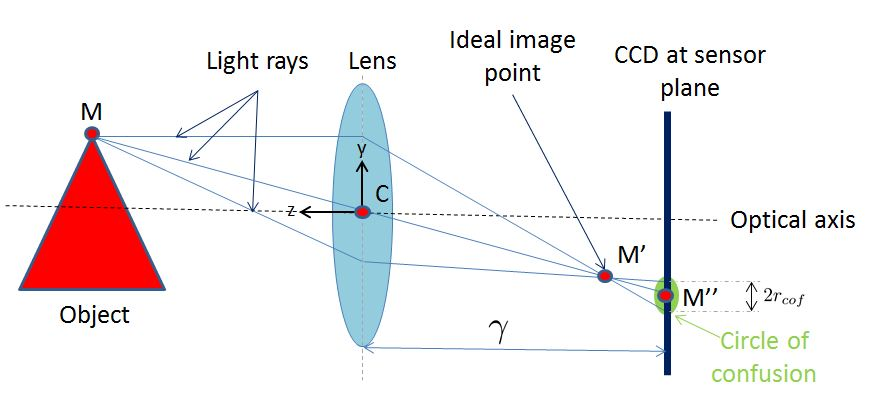
\includegraphics[scale=0.6]{Optics}
    \caption{Illustration of how light rays are manipulated by the lens}
    \label{fig:optics}
\end{figure}

% Due to the way the lens bends the light rays the image formed if the sensor plane is coincident with the resulting in an inverted image M'' (x'',y'',z'') if the sensor plane is behind the ideal image point. Since this is the most common camera configuration an inverted coordinate system is used for the sensor plane.

The thin lens equation can be stated as
\begin{equation}
\frac{1}{|CM|} + \frac{1}{CM'} = \frac{1}{\mean{f}}
\end{equation}
where $\mean{f}$ is the focal length; an inherent property of the lens. Additionally through similarity of triangles we have
\begin{align}
\frac{y}{CM} = \frac{-y'}{CM'}\\
\frac{x}{CM} = \frac{-x'}{CM'}\\
\frac{z}{CM} = \frac{-z'}{CM'}.
\end{align}
Combining these a series of equations for the ideal image point can be obtained.
\begin{align}
\label{eq:optics y'2y}
\begin{split}
x'&=\frac{-\mean{f} x}{z - \mean{f}} \\
y'&=\frac{-\mean{f} y}{z - \mean{f}} \\
z'&=\frac{-\mean{f} z}{z - \mean{f}}
\end{split}
\end{align}

\subsection{Circle of confusion}
It is impossible to align the sensor plane perfectly with the ideal image points and so the divergence of the light rays after the ideal image point causes the light rays to illuminate a circular area on the sensor plane. This blurred region is known as the circle of confusion. If this circular area is larger than the area spanned by an element of the sensor then this will result in blurring in the image as the light spills over multiple sensors. This blur could be eliminated by having the sensor plane the same distance from the lens as the the ideal image point but different points on the object will have different ideal image points.

The light rays that make up the outer perimeter of the circle of confusion are the rays that pass through the lens on the outer edges. Using these rays it is possible to determine the radius of the circle of confusion. Taking $r$ to be the radius of the lens these outer light rays pass through the midplane of the lens at $[r \cos \beta, r \sin \beta, 0]^T$ where $0<\beta<2\pi$. Using trigonometry the y components of these light rays can be related.
\begin{equation}
	\frac{y' - r \sin \beta}{z'}= \frac{y' - y''}{\gamma + z'}
\end{equation}
Th distance between the lens and the sensor plane is given by $\gamma$. The same can be done for the x component. Using this and equation \ref{eq:optics y'2y} an expression for the perimeter of the circle of confusion can be found.
\begin{equation}
\label{eq:cof}
	\begin{bmatrix}
	x'' \\
	y'' \\
	z''
	\end{bmatrix} =
	\begin{bmatrix}
	r \cos \beta + r \cos \beta \left( 1 + \frac{\gamma \left( \mean{f} - z \right)}{\mean{f} z} \right) \\
	r \sin \beta + r \sin \beta \left( 1 + \frac{\gamma \left( \mean{f} - z \right)}{\mean{f} z} \right) \\
	0
	\end{bmatrix} +
	\begin{bmatrix}
	-\frac{\gamma x}{z} \\
	-\frac{\gamma y}{z} \\
	- \gamma
	\end{bmatrix}
\end{equation}
The radius of the circle of confusion can be determine by taking the difference in the y components of $y''$ for $\beta=90 ^{\circ} $ and $\beta=270 ^{\circ}$.

\begin{align}
	2 r_{cof} &= \left[r \sin 90 ^{\circ} \left( 2 + \frac{\gamma \left( \mean{f} - z \right)}{\mean{f} z} \right) \right] - \left[r \sin 270 ^{\circ} \left( 2 + \frac{\gamma \left( \mean{f} - z \right)}{\mean{f} z} \right) \right] \\
	r_{cof}&=r \left( 1 + \frac{\gamma \left( \mean{f} - z \right)}{\mean{f}z} \right)
\end{align}

Another way that the blur can be improved is by using an aperture. An aperture is at a basic level an opaque diaphragm with a hole in it which serves to reduce the amount of light that is incident upon the sensor. Thus by blocking off the light that passed through the outer edges of the lens the aperture reduces the size of the circle of confusion by effectively reducing the radius of the lens. The aperture can be place in front or behind the lens. 

\subsection{Depth of field}
Depth of field is defined as the distance ahead and behind the object that is in focus. For a particular camera system the ideal image point of an object will fall upon the sensor plane if the object is at an ideal focal length from the lens. If the object is any closer or further from the lens it will cause a circle of confusion on the sensor plane as opposed to a point. If the circle of confusion is small enough it will not spill significant light over multiple sensors which will result in a clear image.% be interpreted as a point by the light sensor in which case it is clear in the image.

However if the circle of confusion is large enough it will cause blurring in the image. The largest circle of confusion which still results in a sharp image is referred to as the acceptable circle of confusion \cite{sutton2009image}. Thus the depth of field can be considered as the distance along the z-axis ahead or behind the ideal focus length which results in an acceptable circle of confusion.

The largest degree of freedom for a specific camera system occurs when the object is at the hyperfocal length, $H$, from the camera. The hyperfocal length is defined as the closest an object can be to the camera such that the depth of field extends to infinity behind the object. In this situation the depth of field starts at a distance of $\frac{H}{2}$. The hyperfocal length can be approximated as
\begin{equation}
	H \simeq \frac{\mean{f}^2}{2 N r_{cof}}
	\label{eq:hyperfocal}
\end{equation}
Here $N$ is given by $\frac{\mean{f}}{D_p}$ where $D_p$ is the diameter of the entrance pupil for the camera system. Letting $s$ be the distance from the camera to the object such that the camera is ideally focused at a distance $s$. The distance from the camera to the near limit of the depth of field, $D_N$, and the distance from the camera to the far limit of the depth of field, $D_F$, can be approximated.
\begin{align}
	D_N \simeq \frac{Hs}{H+s} \\
	D_F \simeq \frac{Hs}{H-s}
\end{align}
These approximations assume that the object distance is large compared to the lens focal length. The depth of field can then be determined.
\begin{equation}
	DOF = D_F - D_N = \frac{2 H s^2}{H^2 - s^2}
	\label{eq:DOF}
\end{equation}
Combining equation \ref{eq:hyperfocal} and \ref{eq:DOF} 
\begin{equation}
	DOF = \frac{4 N r_{cof} \mean{f}^2 s^2}{\mean{f}^4 - 4 N^2 r_{cof}^2 s^2}.
\end{equation}
Thus it is clear that the depth of field can be controlled by altering the focal length of the lens, by altering $N$ by changing the aperture or changing the distance between the camera and the object.

\subsection{Field of view}
\todo{viewing frustum}
The field of view is the extent of the world that the camera is capable of capturing in an image. It is quantified as the largest angle that a light ray, that is incident upon the sensor, makes with the optical axis. This angle is referred to as the angle-of-view.

Using the pinhole camera model with a distance of $L$ between the sensor and the lens and taking the lens height to be $d$ a relation for the angle-of-view, $\alpha$, can be derived using trigonometry.
\begin{align}
	\tan \left( \frac{\alpha}{2} \right) &= \frac{d}{2 L} \\
	\alpha &= 2 \arctan \left( \frac{d}{2L} \right)
\end{align}

However for the best picture quality the distance between the sensor and the lens should be equal to the focal length $f$.
\begin{equation}
	\alpha = 2 \arctan \left( \frac{d}{2f} \right)
\end{equation}

\subsection{Transformation to image plane}
The relation between an object point and the projection of the object point onto the sensor can be derived from equation \ref{eq:cof} by eliminating the circle of confusion component. Additionally when the camera system is set up properly $z'$ will be equal to $\gamma$ so that the sensor plane is approximately coincident with the ideal image points. 
\begin{equation}
\label{eq:w2i}
	\begin{bmatrix}
	x'' \\
	y'' \\
	z''
	\end{bmatrix} = 
	\begin{bmatrix}
	-\frac{\gamma}{z} & 0 & 0 \\
	0 & -\frac{\gamma}{z} & 0 \\
	0 & 0 & -\gamma
	\end{bmatrix}
	\begin{bmatrix}
	x \\
	y \\
	1
	\end{bmatrix}
\end{equation}
This equation presents two issues. Firstly the dependence of the sensor positions on $z$. Secondly all the terms in the equation have metric units whereas the image coordinate system has dimensions measured in pixels. These issues are fixed by using a homogeneous from of equation \ref{eq:w2i}.
\begin{equation}
\label{eq:w2ih}
	\alpha \begin{bmatrix}
	-x'' \\
	-y'' \\
	1
	\end{bmatrix} =
	\begin{bmatrix}
	\gamma & 0 & 0 & 0 \\
	0 & \gamma & 0 & 0 \\
	0 & 0 & 1 & 0
	\end{bmatrix}
	\begin{bmatrix}
	x \\
	y \\
	z \\
	1
	\end{bmatrix}
\end{equation}
Here $\alpha$ is a scale factor which allows for the conversion from metric units for the world coordinate system to pixels used in the sensor coordinate system. This equation is referred to as perspective projection \cite{sutton2009image}.

\subsection{Front image plane model}
A new imaging model that is often preferred for computer vision applications can be obtained by translating the sensor plane a distance of $2\gamma$ along the optical axis. In this case the sensor plane is in front of the lens. Treating the sensor coordinates $M''$ of an object as the intersection of the light ray with the sensor plane; equation \ref{eq:w2ih} remains valid for this configuration.

This imaging model is advantageous in that the sensor plane coordinates are no longer inverted. This means that the scene being imaged is also not inverted.

% \begin{itemize}
% 	\item intro
% 	\item circle of confusion
% 	\item M to M''
% 	\item aperture
% 	\item DOF
% 	\item angle of view
% 	\item pinhole inversion
% \end{itemize}

% The surfaces are convex such that diffuse light emanating from a point on an object that passes through the lens will converge and intersect at a point called the ideal imaging point. After the ideal imaging point the light rays begin to diverge again. Once this divergence occurs the image becomes inverted. The lens is placed in front of the sensor plane in an attempt to focus the light from each part of the object onto a single light sensor.

% Lenses are usually disk shaped pieces of glass with two convex surfaces. The surfaces are convex such that diffuse light emanating from a point on an object that passes through the lens will converge and intersect at a point called the ideal imaging point. After the ideal imaging point the light rays begin to diverge again. Once this divergence occurs the image becomes inverted. The lens is placed in front of the sensor plane in an attempt to focus the light from each part of the object onto a single light sensor.

% This is illustrated in figure \todo{figure}.

%  which refract light that passes through them to bring the light closer to the usually shaped such that they have convex surfaces that are shaped in such a way that light passing through the lens is refracted towards the optical axis such that  
\section{Coordinate systems}
\label{sec:coord sys}
Images are only capable of storing two dimensional information whereas we live in a three dimensional world. Thus cameras convert three dimensional information from the world coordinate system into two dimensional information in the sensor coordinate system when a picture is taken as shown in figure \ref{fig:coordsys}. The mathematical relationship between these two coordinate systems is discussed here.

\begin{figure}[h]
    \centering
    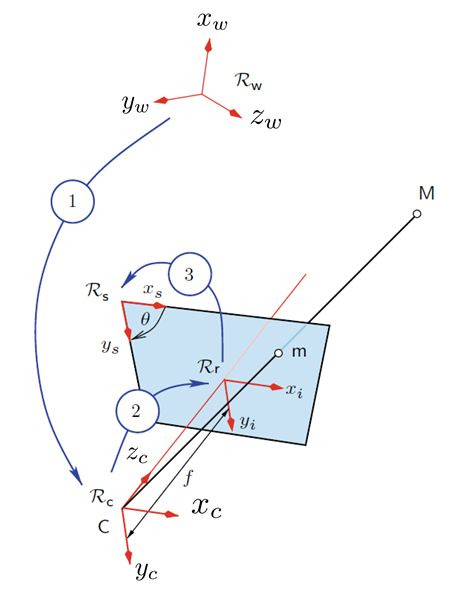
\includegraphics[scale=0.5]{CoordinateSystems}
    \caption{The conversion between coordinate systems that occurs when an image is taken}
    \label{fig:coordsys}
\end{figure}
% Throughout this project thin lenses are assumed. A thin lens is one in which its thickness is negligible in comparison with its focal length or radius of curvature. Additionally the paraxial approximation is assumed which states that light rays passing through the lens do so with a small angle to the lens's optical axis and pass through the lens close to the optical axis. This leads to the small angle approximation.
% \begin{equation}
% 	\sin(\theta) \approx \tan(\theta) \approx \theta
% \end{equation}
\todo[inline]{describe how homogeneous coordinates allow n dim vectors to be manipulated in n+1 dim space}
\subsection{Homogeneous coordinates}
It is common knowledge that any object's shape can be fully defined using distances and angles in 3D Euclidean space. However when an image is taken of this object these distances and angles become distorted. For example railway tracks consist of two beams that remain parallel to one another at a set distance apart in Euclidean space but in an image of the railway track (projective space) these beams appear to get closer and closer to one another as seen in figure \ref{fig:traintrack}. Therefore the parallelism between the beams in Euclidean space is distorted in projective space. This occurs as a result of reducing 3D information to a 2D image. \todo{add image}

\begin{figure}[h]
    \centering
    
\includegraphics[scale=0.1]{TrainTrack}
    \caption{How projective space distorts parallelism present in Euclidean space}
    \label{fig:traintrack}
\end{figure}

Homogeneous coordinates make it possible to take a 3D coordinate in Euclidean space into a 4D coordinate in projective space. This is necessary since a transformation matrix for 3D coordinates that applies both rotation and translation has 4 columns and so can only be applied to a 4D coordinate. Conversion to homogeneous coordinates involves adding an additional coordinate $w$ to the coordinate vector and setting $w=1$. To convert back from homogeneous coordinates requires dividing the $x$, $y$ and $z$ coordinates by $w$ and then eliminating $w$.

\todo{do a 2D example}
% http://www.songho.ca/math/homogeneous/homogeneous.html
% http://www.tomdalling.com/blog/modern-opengl/explaining-homogenous-coordinates-and-projective-geometry/
\subsection{World to camera coordinate system}
Converting from the world coordinate system to the camera coordinate system involves rigid transformations of translation $T$ and rotation $R$. The world coordinate system is simply the coordinate system that would be used to classify the position and orientation of objects in the real world. The world coordinate systems orientation and origin is somewhat arbitrary and it is usually classified according to the object to be imaged. 

The camera coordinate system is as the name suggests fixed according to the cameras position and orientation. The camera coordinate system's z axis is the optical axis of the camera. The conversion between the two coordinate systems can be represented as
\begin{equation}
	\bm{X}_c = 
	\begin{bmatrix}
	x_c \\
	y_c \\
	z_c \\
	1
	\end{bmatrix}
	=
	\begin{bmatrix}
	r_{11} & r_{12} & r_{13} & t_1 \\
	r_{21} & r_{22} & r_{23} & t_2 \\
	r_{31} & r_{32} & r_{33} & t_3 \\
	0 & 0 & 0 & 1
	\end{bmatrix}
	\begin{bmatrix}
	x_w \\
	y_w \\
	z_w \\
	1
	\end{bmatrix} = 
	\begin{bmatrix}
	\bm{R} & \bm{T} \\
	\bm{0} & 1
	\end{bmatrix} \bm{X}_w.
\end{equation}
\todo{change T and R to lowercase}
Scaling of dimensions between the two coordinate systems also needs to be taken into account. The parameters in $\bm{R}$ and $\bm{T}$ are referred to as extrinsic parameters since they are not dependent on the camera system's hardware but rather the camera's position and orientation in the world coordinate system.

\subsection{Camera and imaging plane coordinates}
The 3D object defined in the camera coordinate system is converted to its projection on imaging plane. This conversion is from a 3D coordinate system to a 2D coordinate system as given below using homogeneous coordinates.
\begin{equation}
\label{eq:c2i}
	\bm{X}_i = \alpha
	\begin{bmatrix}
	x_i \\
	y_i \\
	1
	\end{bmatrix} 
	= 
	\begin{bmatrix}
	\gamma & 0 & 0 & 0 \\
	0 & \gamma & 0 & 0 \\
	0 & 0 & 1 & 0
	\end{bmatrix}
	\begin{bmatrix}
	x_c \\
	y_c \\
	z_c \\
	1
	\end{bmatrix}
\end{equation}
The variable $\alpha$ is an arbitrary scale factor.

\subsection{Image plane and sensor coordinates}
At this point the locations of where the light rays originating from the object will intersect the imaging plane are known. Now it is necessary to mathematically represent how the sensor would interpret these light rays incident upon the sensor into the form of pixels. In order to do this a relation between the position of a point within a coordinate system and the pixel within an image is necessary. Additionally the sensor array is not guaranteed to the orthogonal and so a skewed coordinate system must be taken into account.

The transformation from the image plane coordinate system to a temporary skewed coordinate system with an angle of $\phi$ between the two axes can be represented by
\begin{equation}
\label{eq:plane2skew}
	\begin{bmatrix}
	x_{temp} \\
	y_{temp} 
	\end{bmatrix} =
	\begin{bmatrix}
	1 & -\cot \phi \\
	0 & \frac{1}{\sin \phi}
	\end{bmatrix}
	\begin{bmatrix}
	x_i\\
	y_i
	\end{bmatrix}.
\end{equation}
It is assumed that the two principle directions in the sensor coordinate system have different scale factors, $S_x$ and $S_y$,which have units of pixels per unit length. Applying these to the coordinates calculated in equation \ref{eq:plane2skew} and accounting for the translations $\hat c_x$ and $\hat c_y$ to convert to the origin of the sensor coordinate system results in the sensor coordinates below.
\begin{equation}
	\begin{bmatrix}
	x_s \\
	y_s
	\end{bmatrix} = 
	\begin{bmatrix}
	S_x & 0\\
	0 & S_y
	\end{bmatrix}
	\begin{bmatrix}
	x_{temp}\\
	y_{temp}
	\end{bmatrix} -
	\begin{bmatrix}
	S_x \hat c_x - S_x \hat c_y \cot \phi \\
	\frac{S_y \hat c_y}{\sin \phi}
	\end{bmatrix}=
	\begin{bmatrix}
	S_x & -S_x \cot \phi \\
	0 & \frac{S_y}{\sin \phi}
	\end{bmatrix}
	\begin{bmatrix}
	x_i \\
	y_i
	\end{bmatrix} -
	\begin{bmatrix}
	S_x \hat c_x - S_x \hat c_y \cot \phi \\
	\frac{S_y \hat c_y}{\sin \phi}
	\end{bmatrix}
\end{equation}

This can be rewritten in homogeneous form so that it is consistent with equation \ref{eq:c2i}.
\begin{equation}
	\bm{X}_s = 
	\begin{bmatrix}
	x_s \\
	y_s \\
	1
	\end{bmatrix} =
	\begin{bmatrix}
	S_x & -S_x \cot \phi & -S_x \left( \hat c_x - \hat c_y \cot \phi \right) \\
	0 & \frac{S_y}{\sin \phi} & -\frac{S_y \hat c_y}{\sin \phi} \\
	0 & 0 & 1
	\end{bmatrix}
	\begin{bmatrix}
	x_i \\
	y_i \\
	1
	\end{bmatrix} =
	\bm{A} \bm{X}_i
\end{equation}
\todo{talk about these parameters being intrinsic and combine them better}

\subsection{World to sensor coordinates}
The conversions between coordinate systems described in the previous sections can be combined into one conversion from the world coordinate system to the sensor coordinate system.
\begin{equation}
	\bm{X}_s = \alpha
	\begin{bmatrix}
	x_s \\
	y_s \\
	1
	\end{bmatrix} =
	\begin{bmatrix}
	S_x & -S_x \cot \phi & -S_x \left( \hat c_x - \hat c_y \cot \phi \right) \\
	0 & \frac{S_y}{\sin \phi} & -\frac{S_y \hat c_y}{\sin \phi} \\
	0 & 0 & 1
	\end{bmatrix}
	\begin{bmatrix}
	\gamma & 0 & 0 & 0 \\
	0 & \gamma & 0 & 0 \\
	0 & 0 & 1 & 0
	\end{bmatrix}
	\begin{bmatrix}
	r_{11} & r_{12} & r_{13} & t_1 \\
	r_{21} & r_{22} & r_{23} & t_2 \\
	r_{31} & r_{32} & r_{33} & t_3 \\
	0 & 0 & 0 & 1
	\end{bmatrix}
	\begin{bmatrix}
	x_w \\
	y_w \\
	z_w \\
	1
	\end{bmatrix}
\end{equation}

This can be simplified by combining the first two matrices.
\begin{align}
	\bm{X}_s = \alpha
	\begin{bmatrix}
	x_s \\
	y_s \\
	1
	\end{bmatrix} =
	\begin{bmatrix}
	\gamma S_x & -\gamma S_x \cot \phi & -S_x \left( \hat c_x - \hat c_y \cot \phi \right) & 0\\
	0 & \frac{\gamma S_y}{\sin \phi} & -\frac{S_y \hat c_y}{\sin \phi} & 0\\
	0 & 0 & 1 & 0
	\end{bmatrix}
	\begin{bmatrix}
	r_{11} & r_{12} & r_{13} & t_1 \\
	r_{21} & r_{22} & r_{23} & t_2 \\
	r_{31} & r_{32} & r_{33} & t_3 \\
	0 & 0 & 0 & 1
	\end{bmatrix}
	\begin{bmatrix}
	x_w \\
	y_w \\
	z_w \\
	1
	\end{bmatrix}
	\label{eq:world 2 sensor cumbersome}
\end{align}

Replacing the elements of the first matrix in equation \ref{eq:world 2 sensor cumbersome} with single variables for the purposes of simplicity the equation can be rewritten as

\begin{align}
	\alpha
	\begin{bmatrix}
	x_s \\
	y_s \\
	1
	\end{bmatrix} &=
	\begin{bmatrix}
	f_x & f_s & c_x & 0\\
	0 & f_y & c_y & 0\\
	0 & 0 & 1 & 0
	\end{bmatrix}
	\begin{bmatrix}
	r_{11} & r_{12} & r_{13} & t_1 \\
	r_{21} & r_{22} & r_{23} & t_2 \\
	r_{31} & r_{32} & r_{33} & t_3 \\
	0 & 0 & 0 & 1
	\end{bmatrix}
	\begin{bmatrix}
	x_w \\
	y_w \\
	z_w \\
	1
	\end{bmatrix} \\
	&= \bm{K} \bm{V} \bm{X}_w.
	\label{eq:world 2 sensor}
\end{align}
Here the parameters relating the world coordinate system to the sensor coordinate system are separated into two matrices. The first matrix $\bm{K}$ contains the intrinsic parameters which are fixed for a specific camera. The second matrix $\bm{V}$ contains the extrinsic parameters. The extrinsic parameters change when the camera's position and orientation relative to the world coordinate system changes.
\todo{explain this better}

\section{Distortion}
Distortion refers to a collection of phenomena that cause the actual image to differ from that of the idealised image expected from the pinhole camera model. This happens because lenses cannot be manufactured and assembled perfectly and so some misalignment and defects exist in the imaging system. Therefore in order to calculate accurate displacement information the distortions must be accounted for and corrected prior to the correlation process.

Distortion can be separated into many types as done below. The overall distortion of the image can then be mathematically represented as the linear combination of the mathematical expressions for the individual types. A brief explanation of each distortion type and the equation that accounts for the distortion it creates is given below.
% https://www.lensrentals.com/blog/2010/10/the-seven-deadly-aberrations/

\subsection{Spherical distortion}
Spherical distortion is when light rays originating from a point on an object intersect at different points on the sensor plane. This is as a result of the lens not having the perfect curvature required for all the light rays to intersect at the same point on the sensor plane. It is assumed to be axis symmetric relative to the axis passing through the centre of the sensor and to be a function of the radial distance.
\begin{equation}
	\bm{D} = \kappa_1 \rho ^4 \bm{e}_r
\end{equation}
Here $\bm{e}_r$ is the radial unit vector and $\rho$ is the distance from the origin of the sensor coordinate system to the point under consideration.

\subsection{Coma distortion}
Coma distortion affects light rays that travel towards the lens at an angle to the optical axis. Light rays that go through the centre portion of lens refocus to a point on the sensor plane, whereas light rays that pass through the outer portion of the lens don't refocus fully and intersect the sensor plane further (positive coma) or closer (negative coma) to the optical axis. This results in light from a point on an object creating a comet-like shape on the sensor plane. It is corrected with the following equation.
\begin{equation}
	\bm{D} = \kappa_2 \rho^3 \cos \left( \mean{\theta} - \mean{\theta_c} \right) \bm{e}_r
\end{equation}
Here $\mean{\theta_c}$ is the orientation of the projected lens tilt angle in the sensor plane.

\subsection{Astigmatism}
Astigmatism is caused by a lens having curvature that varies when measured along perpendicular planes. For instance the vertical plane of the lens has a different curvature to the horizontal plane of the lens. The different curvatures have different focal lengths and so light passing through the vertical portion of the lens will focus at a different distance from the lens than light that passes through the horizontal portion of the lens. This results in line like blurs on the sensor plane for the curvature that is not in focus. The degree to which the astigmatism affects the image increases further away from the centre of the image.
\begin{equation}
	\bm{D} = \kappa_3 \rho^2 \cos \left( \mean{\theta} - \mean{\theta}_A \right) \bm{e}_r
\end{equation}
Where $\mean{\theta}_A$ is the orientation of the projected astigmatic plane within the sensor plane.

\subsection{Curvature of field}
Curvature of field is a distortion that results due to the curved nature of the optical elements such as the lens. As light rays pass through the lens with a small angle to the optical axis they refocus at the sensor plane. However light rays that pass through the lens at a larger angle to the optical axis refocus at a point that is closer to the lens. This results in the light rays refocusing on a curved plane much like a shallow dome. Since the sensor is planar (flat) this causes the centre of the image to be in focus while the edges of the image are not in focus.

Curvature of field is assumed to be symmetric with respect to the optical axis and to be a quadratic function of the radial position \cite{sutton2009image}.
\begin{equation}
	\bm{D}=\kappa_4 \rho^2 \bm{e}_r
\end{equation}
Here $\kappa_4$ is the amplitude of the curvature of distortion in the sensor plane measured in $\text{pixels}^{-1}$.
% https://photographylife.com/what-is-field-curvature

\subsection{Linear}
This non-symmetric distortion component is assumed to be a linear function of radial position and is dependent on the angular position \cite{sutton2009image}.
\begin{equation}
	\bm{D} = \kappa_5 \rho \cos \left( \mean{\theta} - \mean{\theta_L} \right) \bm{e}_r
\end{equation}
Here $\mean{\theta_L}$ is the angular orientation of the linear distortion axis.

\subsection{Radial}
Radial distortion is caused by the lens having different magnification levels based on the angle of the light rays to the optical axis. As a result the image can experience a decrease in magnification with increasing distance from the optical axis (barrel distortion) or the image can experience increasing magnification with increasing distance from the optical axis (pincushion distortion). This distortion is symmetric with respect to the optical axis.
\begin{equation}
	\bm{D} = \kappa_6 \rho ^3 \bm{e}_r + \kappa_7 \rho^5 \bm{e}_r + \kappa_8 \rho^7 \bm{e}_r
\end{equation}
% http://www.shariblog.com/2013/08/difference-between-barrel-pincushion-distortion/
% https://photographylife.com/what-is-distortion
\subsection{De-centering}
De-centering distortion is caused by the lens not being in perfect alignment with the rest of the camera system. Usually this type of distortion is less severe than radial or spherical distortions.
\begin{equation}
	\bm{D} = \kappa_9 \rho^2 \left[ 3 \sin \left( \mean{\theta} - \mean{\theta_d} \right) \bm{e}_r + \cos \left( \mean{\theta} - \mean{\theta_d} \right) \bm{e}_t \right]
\end{equation}
Here $\bm{e}_t$ is the tangential unit vector and $\mean{\theta_d}$ is the orientation of the axis for maximum tangential distortion.

% http://www.pcigeomatics.com/geomatica-help/concepts/orthoengine_c/Chapter_47.html
\section{Calibration}
Calibration is a necessary process that must be completed in order to extract metric information from images. The calibration process solves for parameters that define the optical characteristics of the camera, parameters that define the orientation and position of the camera coordinate system to the world coordinate system and parameters that define the distortions that must be corrected in the images. 

The parameters that define the optical characteristics and the distortions are referred to as intrinsic parameters since they are fixed for a specific camera. The parameters that describe the orientation and position of the camera within the world coordinate system are extrinsic parameters because they change if the camera is moved. \todo{explain intrinsic and extrinsic better}

Multiple methods of calibration exist however calibration using a calibration plate is used in this project since it is one of the most popular methods and making a calibration plate is relatively simple and inexpensive. Calibration for distortion parameters will not be focused on in this section. \todo{take out distortion not used}

\subsection{Inverse problem}
Calibration is essentially a method of finding the parameters that allow 3D coordinates in the world coordinate system to be accurately related to 2D coordinates in the image coordinate system. Thus the inputs, 3D world coordinates, and outputs, 2D image coordinates, needed to be used to solve for the parameters which describe the relationship between the two which constitutes an inverse problem.

Inverse problems are typlically hard to solve and calibration is no exception. In order to solve for the calibration parameters more reliably the camera model that relates world points to sensor points is broken down to the simple pinhole camera model initially in order to solve for as few parameters as possible initially. These parameters are solved for using a closed form solution which gives good estimates to the parameters. Thereafter once these parameters have been estimated the camera model is made more complex by introducing radial distortion in order to account for imperfections in the lens system of the camera. These radial parameters are first estimated and once each parameter has a corresponding estimate all the parameters are optimized in an iterative manner.

This inverse problem is sensitive to errors in the 3D world coordinates (inputs) and 2D image coordinates (outputs) used. Thus these need to be known to a high degree of accuracy in order to solve for the intrinsic and extrinsic camera parameters reliably. This is achieved by using a calibration plate.

\subsection{Calibration plate}
A calibration plate is an object with a flat surface containing a high-contrast, regular pattern. The pattern is such that it contains definitive, point-like features which can be located to a high degree of accuracy within images taken of it. For example a checker board pattern allows for accurate calculation of the points at the corners of the squares. Thus the coordinates of these point-like features on the calibration plate will be known (inputs) and the coordinates of these point-like features in the image can be determined to a high degree of accuracy (outputs).

Since images inherently contain some level of noise it is best to have an overdetermined system of equations. This is accomplished by taking multiple images of the calibration plate and changing the relative position and orientation between the calibration plate and the camera for each image. This effectively reduces the effects of noise; making the system more robust.

\subsection{Homography}
\label{sec: homography}
Homography is a transformation that can be applied to points on a plane to bring it into alignment with another plane. It is used to bring the points on the calibration plate in the world coordinate system into alignment with their location in the image in the sensor coordinate system. The transformation from world coordinates to sensor coordinates in equation \ref{eq:world 2 sensor} is a type of homography.

Treating the calibration plate such that it lies in the x-y plane of the world coordinate system; the homography, $\bm{H}$, for calibration is given by the following equation.
\begin{equation}
	\begin{bmatrix}
	x_s \\
	y_s \\
	1
	\end{bmatrix} = 
	\alpha
	\begin{bmatrix}
	f_x & f_s & c_x & 0\\
	0 & f_y & c_y & 0\\
	0 & 0 & 1 & 0
	\end{bmatrix}
	\begin{bmatrix}
	r_{11} & r_{12} & r_{13} & t_1 \\
	r_{21} & r_{22} & r_{23} & t_2 \\
	r_{31} & r_{32} & r_{33} & t_3 \\
	0 & 0 & 0 & 1
	\end{bmatrix}
	\begin{bmatrix}
	x_w \\
	y_w \\
	0 \\
	1
	\end{bmatrix} \\
\end{equation}
This can be reduced to 
\begin{align}
	\begin{bmatrix}
	x_s \\
	y_s \\
	1
	\end{bmatrix} &=
	\alpha
	\begin{bmatrix}
	f_x & f_s & c_x \\
	0 & f_y & c_y \\
	0 & 0 & 1 
	\end{bmatrix}
	\begin{bmatrix}
	r_{11} & r_{12} & t_1 \\
	r_{21} & r_{22} & t_2 \\
	r_{31} & r_{32} & t_3 
	\end{bmatrix}
	\begin{bmatrix}
	x_w \\
	y_w \\
	1
	\end{bmatrix} \\
	&= \alpha \bm{K} 
	\begin{bmatrix}
	\bm{r}_1 & \bm{r}_2 & \bm{t}
	\end{bmatrix}
	\begin{bmatrix}
	x_w \\
	y_w \\
	1
	\end{bmatrix} \\
	&= \alpha
	\begin{bmatrix}
	h_1 & h_2 & h_3 \\
	h_4 & h_5 & h_6 \\
	h_7 & h_8 & h_9
	\end{bmatrix} 
	\begin{bmatrix}
	x_w \\
	y_w \\
	1
	\end{bmatrix}
	=\alpha \bm{H} 
	\begin{bmatrix}
	x_w \\
	y_w \\
	1
	\end{bmatrix} \label{eq: homography 1}
\end{align}
Here $\bm{r}_1$ and $\bm{r}_2$ are the first and second columns of the rotation matrix. It is clear that the homography matrix contains both intrinsic and extrinsic parameters and thus it is different for each image taken of the calibration plate. Additionally note that the homography matrix is defined up to a scale factor.

%http://www.learnopencv.com/homography-examples-using-opencv-python-c/

\subsection{Estimating homography with direct linear transform}
The homographies that relate the world coordinates of the calibration plate targets to the targets in the image can be estimated using direct linear transformation \cite{zhangtut}. Equation \ref{eq: homography 1} can be written out as
\begin{align}
	x_s &= \alpha \left( h_1 x_w + h_2 y_w + h_3 \right) \label{eq: homo line 1} \\
	y_s &= \alpha \left( h_4 x_w + h_5 y_w + h_6 \right) \label{eq: homo line 2} \\
	1 &= \alpha \left( h_7 x_w + h_8 y_w + h_9 \right) \label{eq: homo line 3}.
\end{align}
The scale factor, $\alpha$, can be eliminated by dividing equations \ref{eq: homo line 1} and \ref{eq: homo line 2} by \ref{eq: homo line 3} to get
\begin{align}
	x_s \left( h_7 x_w + h_8 y_w + h_9 \right) &= \left( h_1 x_w + h_2 y_w + h_3 \right) \\
	y_s \left( h_7 x_w + h_8 y_w + h_9 \right) &= \left( h_4 x_w + h_5 y_w + h_6 \right)
\end{align}
These equations then reduce to
\begin{align}
	- h_y x_w x_s - h_8 y_w x_s + h_1 x_w + h_2 y_w +h_3 &= h_9 x_s \label{eq: solve homo 1}\\
	- h_7 x_w y_s - h_8 y_w y_s + h_4 x_w + h_5 y_w + h_6 &= h_9 y_s. \label{eq: solve homo 2}
\end{align}
In order to avoid the trivial solution where every element in the homogrpahy matrix is equal to zero; constraints need to be placed on the elements of the homography matrix. In this case the element $h_9$ is set equal to 1 however other constraints are also possible such as $h_7^2 + h_8^2 + h_9^2 = 1$. Note that if the true value of $h_9$ is close to zero then this assumption will introduce a singluarity \cite{emerging}.

Each target, having points $x_{w_i}$ and $y_{w_i}$, on the calibration plate that is captured within an image of the calibration plate, having points $x_{s_i}$ and $y_{s_i}$, provides both an equation \ref{eq: solve homo 1} and \ref{eq: solve homo 2}. These are then combined into an equation of the form
\begin{align}
	\begin{bmatrix}
	x_{w_1} & y_{w_1} & 1 & 0 & 0 & 0 & -x_{w_1} x_{s_1} & -y_{w_1} x_{s_1} \\
	0 & 0 & 0 & x_{w_1} & y_{w_1} & 1 & -x_{w_1} y_{s_1} & -y_{w_1} y_{s_1} \\
	x_{w_2} & y_{w_2} & 1 & 0 & 0 & 0 & -x_{w_2} x_{s_2} & -y_{w_2} x_{s_2} \\
	0 & 0 & 0 & x_{w_2} & y_{w_2} & 1 & -x_{w_2} y_{s_2} & -y_{w_2} y_{s_2} \\
	\vdots & \vdots & \vdots & \vdots & \vdots & \vdots & \vdots & \vdots 
	\end{bmatrix}
	\begin{bmatrix}
	h_1 \\
	h_2 \\
	h_3 \\
	h_4 \\
	h_5 \\
	h_6 \\
	h_7 \\
	h_8
	\end{bmatrix} =
	\begin{bmatrix}
	x_{s_1} \\
	y_{s_1} \\
	x_{s_2} \\
	y_{s_2} \\
	\vdots
	\end{bmatrix}
\end{align}
This overdetermined system of equations then can be used to solve for the homography matrices of each calibration image using least squares. This is the first step involved in calibration. \todo{speak about normalisation}

\subsection{Absolute conic}
\label{sec: abs conic}
As mentioned before two objects that are parallel in Euclidean space appear to intersect each other in projective space. The intersection of these two lines in projective space occurs at a point that lies on the plane at infinity. If a point lies upon the plane at infinity its $w$ is equal to zero in homogeneous coordinates.

The absolute conic lies on the plane at infinity and is defined by the set of points, $\tilde{\bm{x}}_{ac} = [x, y, z, w]^T$, that satisfies the following. 
\begin{align}
	w = 0 \\
	\bm{x}_{ac}^T \bm{x}_{ac}=x^2 + y^2 + z^2 = 0 
	\label{eq:conditions of absolute conic}
\end{align}
Here tilde is used to indicate homogeneous coordinates whereas $\bm{x}_{ac} = [x, y, z]^T$ would be the point in Euclidean space.

Thus it is the conic of purely imaginary points that lies upon the plane at infinity. The importance of the absolute conic is that it is invariant under any Euclidean transformations. In other words the relative position of the absolute conic to a moving camera is unaffected by extrinsic parameters. Consider a point $\bm{x}_{ac}$ in Euclidean space in the world coordinate system that lies on the absolute conic. It has homogeneous coordinates $\tilde{\bm{x}}_{ac}=[\bm{x}_{ac}^T, 0]^T$ in projective space. Applying a different rotation and translation to this point to obtain $\tilde{\bm{x}}_{ac}'$, which is equivalent to moving the camera in the world coordinate system, a corresponding point is obtained in the camera coordinate system.
\begin{align}
	\tilde{\bm{x}}_{ac}' &=
	\begin{bmatrix}
	\bm{R} & \bm{T} \\
	\bm{0} & 1
	\end{bmatrix}
	\tilde{\bm{x}}_{ac} =
	\begin{bmatrix}
	r_{11} & r_{12} & r_{13} & t_1 \\
	r_{21} & r_{22} & r_{23} & t_2 \\
	r_{31} & r_{32} & r_{33} & t_3 \\
	0 & 0 & 0 & 1
	\end{bmatrix}
	\begin{bmatrix}
	x_{ac} \\
	y_{ac} \\
	z_{ac} \\
	0
	\end{bmatrix} \\
	&= 
	\begin{bmatrix}
	\bm{R} \bm{x}_{ac} \\
	0
	\end{bmatrix}
\end{align}
It is clear that this point still lies on the plane at infinity since its $w$ is equal to zero. More importantly it can be proven that this point $\bm{x}_{ac}'$ is on the same absolute conic.
\begin{equation}
	\bm{x}_{ac}'^T \bm{x}_{ac}' = \left( \bm{R} \bm{x}_{ac} \right) ^T \left( \bm{R} \bm{x}_{ac} \right) = \bm{x}_{ac}^T \bm{R}^T \bm{R} \bm{x}_{ac} = \bm{x}_{ac}^T \bm{x}_{ac} = 0
\end{equation}
Thus the absolute conic is invariant to Euclidean transformations. Now consider again a point, $\bm{x}_{ac}$, lying on the absolute conic. The corresponding point, $\bm{m}_s$, in the sensor plane is given by
\begin{align}
	\tilde{\bm{m}}_s &= \frac{1}{\alpha} \bm{K} 
	\begin{bmatrix}
	\bm{R} & \bm{T} \\
	\bm{0} & 1
	\end{bmatrix}
	\begin{bmatrix}
	\bm{x}_{ac} \\
	0
	\end{bmatrix} = \frac{1}{\alpha} \bm{K}
	\begin{bmatrix}
	\bm{R} \bm{x}_{ac} \\
	0
	\end{bmatrix} \\
	\therefore \bm{m}_s &= \frac{1}{\alpha} \bm{K} \bm{R} \bm{x}_{ac}.
\end{align}
Checking whether this point satisfies equation \ref{eq:conditions of absolute conic} results in
\begin{equation}
	\bm{m}_s^T \bm{K}^{-T} \bm{K}^{-1} \bm{m}_s = \frac{1}{\alpha^2} \bm{x}_{ac}^T \bm{R}^T \bm{R} \bm{x}_{ac} = \frac{1}{\alpha^2} \bm{x}_{ac}^T \bm{x}_{ac} = 0
\end{equation}
Thus the image of the absolute conic is itself an imaginary conic. The image of the absolute conic is defined by $\bm{K}^{-T} \bm{K}^{-1}$ \cite{luong1997self}. Thus since the image of the absolute conic is dependent only on intrinsic camera parameters it can be used to solve for the intrinsic camera parameters.

% http://www.cs.unc.edu/~marc/tutorial/node87.html
\subsection{Constraints on intrinsic parameters}
\label{sec: intrinsic constraints}
According to Zhang \cite{emerging} there are two constraints placed upon the intrinsic parameters of the camera. These are important later on in the solving for these intrinsic parameters. The plane of the calibration plate in the camera coordinate system is given by \cite{emerging} 
\begin{equation}
	\begin{bmatrix}
	\bm{r}_3 \\
	\bm{r}_3^T \bm{t}
	\end{bmatrix}^T
	\begin{bmatrix}
	x \\
	y \\
	z \\
	w
	\end{bmatrix} = 0.
\end{equation}
Here $w$ is zero for points on the plane at infinity and one for those that are not. This plane intersects the plane at infinity on a line and it happens that $[\bm{r}_1^T, 0]^T$ and $[\bm{r}_2^T, 0]^T$ are points on this line \cite{emerging}. Thus it is known that any point on this line, $x_c^{\infty}$, is a linear combination of these two points.
\begin{equation}
	x_c^{\infty} = a \begin{bmatrix}
	\bm{r}_1 \\
	0
	\end{bmatrix} + b
	\begin{bmatrix}
	\bm{r}_2 \\
	0
	\end{bmatrix} =
	\begin{bmatrix}
	a \bm{r}_1 + b \bm{r}_2 \\
	0
	\end{bmatrix}
\end{equation}
Now assume that this point, $x_c^{\infty}$, lies on the absolute conic. Then this point must satisfy equation \ref{eq:conditions of absolute conic}. This would require that $a^2+b^2=0$ which results in the solution $b=\pm a i$, where $i=\sqrt{-1}$. As a result it can be seen that the two points along this line intersect the absolute conic at
\begin{equation}
	x_c^{\infty} = a 
	\begin{bmatrix}
	\bm{r}_1 \pm i \bm{r_2} \\
	0
	\end{bmatrix}.
\end{equation}
Since these points lie on the absolute conic they are invariant under Euclidean transformations. Their projection, up to a scale factor, in the sensor coordinate system is given by
\begin{equation}
	x_s^{\infty} = \bm{K} \left( \bm{r}_1 \pm \bm{r}_2 \right) = \bm{h}_1 \pm i \bm{h}_2.
\end{equation}
Substituting these points into equation \ref{eq:conditions of absolute conic} results in
\begin{equation}
	\left( \bm{h}_1 \pm i \bm{h}_2 \right)^T \bm{K}^{-T} \bm{K}^{-1} \left( \bm{h}_1 \pm i \bm{h}_2 \right) = 0.
\end{equation}
Requiring both the imaginary and real parts of this equation to equal zero results in two constraints on the intrinsic camera parameters.
\begin{align}
\label{eq:intrinsic constraints}
	\bm{h}_1^T \bm{K}^{-T} \bm{K}^{-1} \bm{h}_2 &= 0 \\
	\bm{h}_1^T \bm{K}^{-T} \bm{K}^{-1} \bm{h}_1 &= \bm{h}_2^T \bm{K}^{-T} \bm{K}^{-1} \bm{h}_2
\end{align}

\subsection{Intrinsic parameters and the absolute conic}
\label{sec: parameters and the absolute conic}
An homography, $\bm{H}$, between the calibration plate and the image of the calibration plate can be estimated. This homography can then be used to solve for the image of the absolute conic. Once the image of the absolute conic is known it can be used to solve for the intrinsic camera parameters. The image of the absolute conic can be represented as
\begin{equation}
	\bm{B} = \bm{K}^{-T} \bm{K}^{-1} = 
	\begin{bmatrix}
	b_{11} & b_{12} & b_{13}\\
	b_{12} & b_{22} & b_{23} \\
	b_{13} & b_{23} & b_{33}
	\end{bmatrix}
\end{equation}
Since $\bm{B}$ is symmetric its contents can be represented by a 6D vector $\bm{b}=[b_{11} b_{12} b_{22} b_{13} b_{23} b_{33}]^T$. Let $\bm{h}_i = [h_{i1} h_{i2} h_{i3}]^T$ to be the i\textsuperscript{th} column of $\bm{H}$. Then
\begin{equation}
	\bm{h}_I^T \bm{B} \bm{h}_j = \bm{v}_{ij} \bm{b}
\end{equation}
where 
\begin{equation}
	\bm{v}_{ij} = [ h_{i1} h_{j1}, h_{i1} h_{j2} + h_{i2} h_{j1}, h_{i2} h_{j2}, h_{i3} h_{j1} + h_{i1} h_{j3}, h_{i3} h_{j2} + h_{i2} h_{j3}, h_{i3} h_{j3}]^T.
\end{equation}
Then equation \ref{eq:intrinsic constraints} can be rewritten as 
\begin{equation}
	\begin{bmatrix} 
	\bm{v}_{12}^T \\
	( \bm{v}_{11} - \bm{v}_{22})^T
	\end{bmatrix} \bm{b} = \bm{0}
\end{equation}
A separate version of this equation exist for each image taken of the calibration plate and these equations can be stacked, in $\bm{V}$, to give
\begin{equation}
	\bm{V}\bm{b}=\bm{0}.
\end{equation}
The solution for $\bm{b}$, up to a scale factor $\lambda$, is known to be the eigenvector of $\bm{V}^T\bm{V}$ associated with the smallest eigenvalue \cite{emerging}. Once b has been determined it can be used to determine the intrinsic parameters of matrix $\bm{K}$. The relation between $\bm{B}$ and $\bm{K}$ is $\bm{B}=\lambda \bm{K}^{-T} \bm{K}^{-1}$. The intrinsic parameters are determined as follows.
\begin{align}
	c_y &= (b_{12} b_{13} - b_{11} b_{23})/(b_{11} b_{22} - b_{12}^2) \\
	\lambda &= b_{33} -(b_{13}^2 + c_y(b_{12} b_{13} - b_{11} b_{23}))/b_{11}\\
	f_x &= \sqrt{\frac{\lambda}{b_{11}}} \\
	f_y &= \sqrt{\frac{\lambda b_{11}}{b_{11} b_{22} - b_{12}^2}} \\
	f_s &= \frac{-b_{12} f_x^2 f_y}{\lambda} \\
	c_x &= \frac{f_s c_y}{f_y} - \frac{b_{13} f_x^2}{\lambda}
\end{align}
Thereafter the extrinsic parameters can be determined.
\begin{align}
	\bm{r}_1 &= \lambda \bm{K}^{-1} \bm{h}_1 \\
	\bm{r}_2 &= \lambda \bm{K}^{-1} \bm{h}_2 \\
	\bm{r}_3 &= \bm{r}_1 \times \bm{r}_2 \\
	\bm{T} &= \lambda \bm{K}^{-1} \bm{h}_3
\end{align}
At this point it is necessary to incorporate distortions and use them to find better approximations for the intrinsic and extrinsic parameters.

\todo{this section is too close to the paper} %a fleixible new technique and reading 1
% by which the optical characteristics of a camera and the relation between its coordinate system and the world coordinate system are determined. It is performed in order to be able to extract \hl{metric} information from images accurately.

\subsection{Closed form solution}
Sections \ref{sec: homography} throught to \ref{sec: parameters and the absolute conic} illustrate that estimates to the intrinsic and extrinsic parameters can be obtained by first determining the homographies for each calibration image, then these can be used to determine the image of the abolute conic which in turn can be used to determine the intrinsic and extrinsic camera parameters. This is closed form solution is the first part of the calibration process

put inverse problem in calibration plate section

explain homography and absolute conic

then explain closed form solution and optimization - give closed form and explain optimization


\subsection{Distortion in Calibration}
The closed form solution given above does not take distortion into account since it is based on the pinhole camera model. It is only once the closed form solution to the extrinsic and intrinsic parameters is optimised that distortion can be accounted for during the calibration process. As already presented, there are many types of distortion that occur when an image is taken. However it is seldom possible to take all of these distortion types into account since the more distortion paramters introduced into the camera model; the more likely the optimization process becomes unstable.

It has been found \todo{add reference for this} that good calibration results can be achieved by taking only radial distortion into accound during calibration \cite{tsai1987versatile,wei1994implicit}. This is beneficial since it is possible to solve for initial guesses to the radial distortion parameters which helps the optimisation process to avoid local minima as a result of the distortion parameters used.

The distortion applied to the points on the image plane is of the form
\begin{align}
	\begin{bmatrix}
	x_{i_{distorted}} \\
	y_{i_{distorted}}
	\end{bmatrix} &=
	1 + k_1 r^2 + k_2 r^4
	\begin{bmatrix}
	x_i \\
	y_i
	\end{bmatrix}\\
	\text{where} \quad \quad r &= \sqrt{x_i^2 + y_i^2}.
\end{align}

At this point the intrinsic and extrinsic parameters have been determined using the pinhole camera model and the error between the predicted calibration plate targets and the actual location of these in the images is attributed to radial distortion \cite{zhangtut}. This error is represented as
\begin{equation}
	d_1 = x_{s_{actual}} - x_{s_{calculated}}
\end{equation}

An undistorted point, $x_i$ is distorted to point $\tilde{x_i}$ according to
\begin{align}
	\tilde{x_i} &= u_c + (x_i-u_c)*(1 + k1 r^2 + k2 r^4) \\
	&= u_c + x_i - u_c + (x_i-u_c)*(1 + k1 r^2 + k2 r^4) \\
	&= x_i + (x_i-u_c)*(1 + k1 r^2 + k2 r^4) \\
	&= x_i + d_{2_i}
\end{align}

The distortion parameters can be estimated by minimizing the difference between $d_1$ and $d_2$. Thus the least squares solution to the overdetermined system is what is needed.


\section{Displacement fields}
In this section some displacement fields are presented in order to illustrate what information DIC and DVC are capable of extracting from image sets.

\subsection{DIC displacement fields}
The figures below show the displacement fields in the region of the crack of a compact tension sample as it is loaded in the y-direction. As such the x-displacement magnitudes are at most 10 \% of the displacements in the y-direction. It becomes clear in analysing these figures that the displacement fields determined by DIC are quite intuitive and can be easily interpreted to understand the deformation that a specimen has undergone.

Additionally these images illustrate the full-field nature of the displacement data that DIC is capable of determining. This coupled with its high accuracy and high spatial resolution makes DIC a very attractive displacement measurement tool.

\begin{figure}[h]
    \centering
    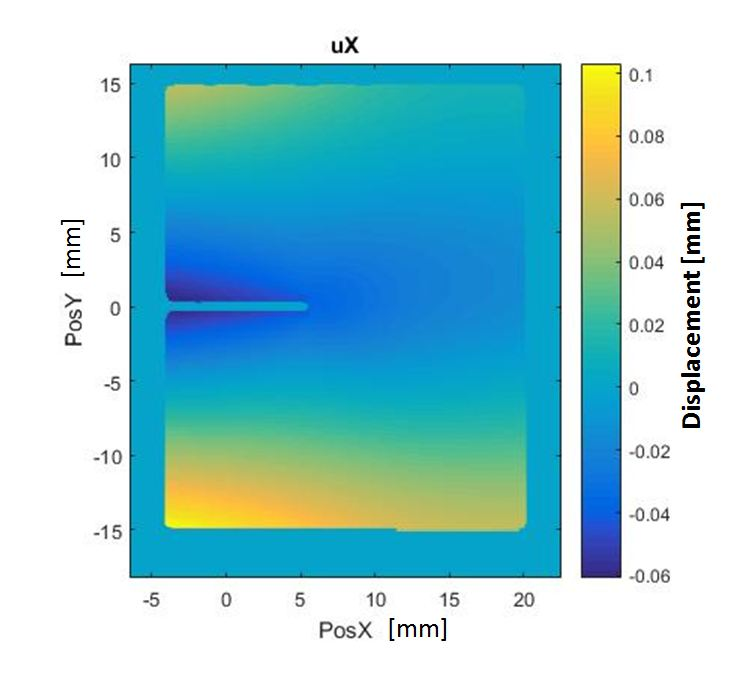
\includegraphics[scale=0.4]{DICuyx}
    \caption{X-direction displacement field of a compact tension specimen (DIC)}
    \label{fig:DICUX}
\end{figure}

\begin{figure}[h]
    \centering
    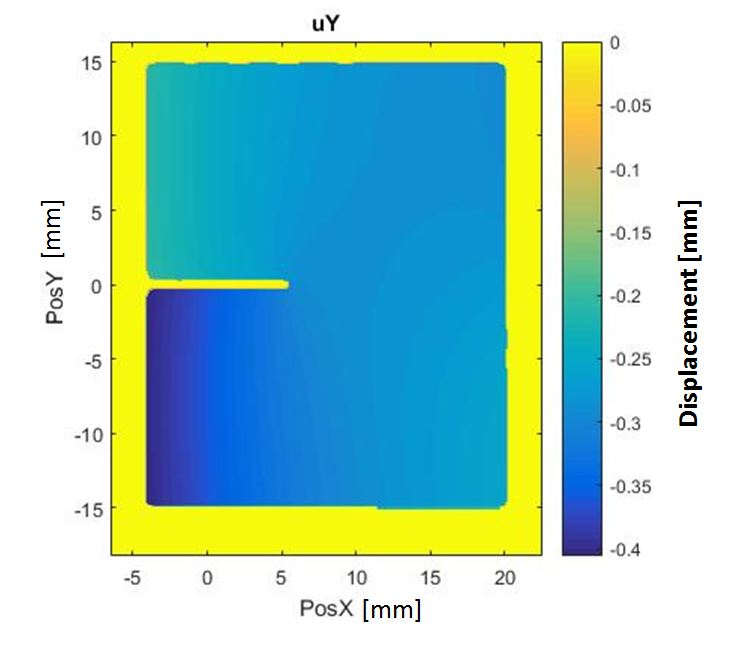
\includegraphics[scale=0.4]{DICuy}
    \caption{Y-direction displacement field of a compact tension specimen (DIC)}
    \label{fig:DICUY}
\end{figure}

\subsection{DVC displacement fields}
DIC displacement fields consist of x and y displacements of points defined in two dimensions. This is because DIC only captures the deformation on the surface of the specimen. However DVC displacement fields consist of x, y and z displacements of points defined in three dimensions. This is because DVC captures deformation information through the thickness of the specimen.

As such in order to visualise DVC displacement fields a plane through the thickness (or on the surface) of the specimen must be chosen. Then the displacements can be visualised on this plane. This plane can then be moved through the thickness of the specimen in order to determine how the displacement fields differ in that direction. 

This is illustrated in figures \ref{fig:DVC1} and \ref{fig:DVC2} by the change in location of the crack front. These figures show the z direction displacement fields of a specimen in the x-y plane at two different heights in the z direction. This is a rectangular specimen that contains a crack front which is not perpendicular to any of the specimens surfaces. These two figures show how the x-y position of the crack front changes with a change in the z position. Thus DVC allows for more of the materials response to be captured.

\begin{figure}[h]
    \centering
    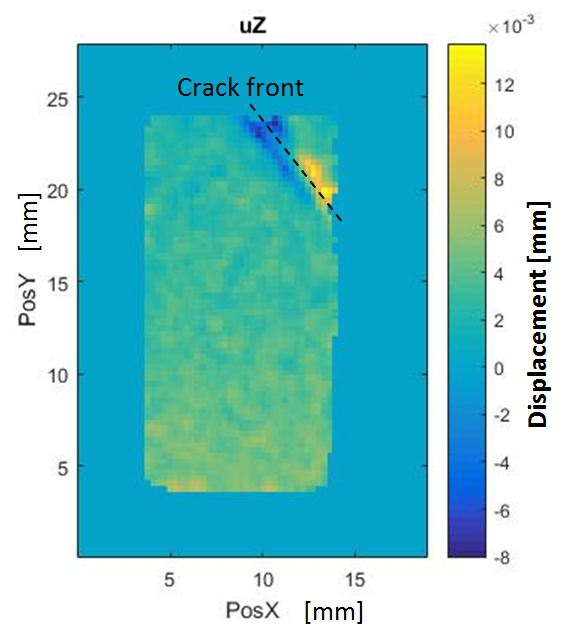
\includegraphics[scale=0.4]{DVC3}
    \caption{Z-direction displacement field on the x-y plane at a height of 13.95 mm in the z direction (DVC)}
    \label{fig:DVC1}
\end{figure}

\begin{figure}[h]
    \centering
    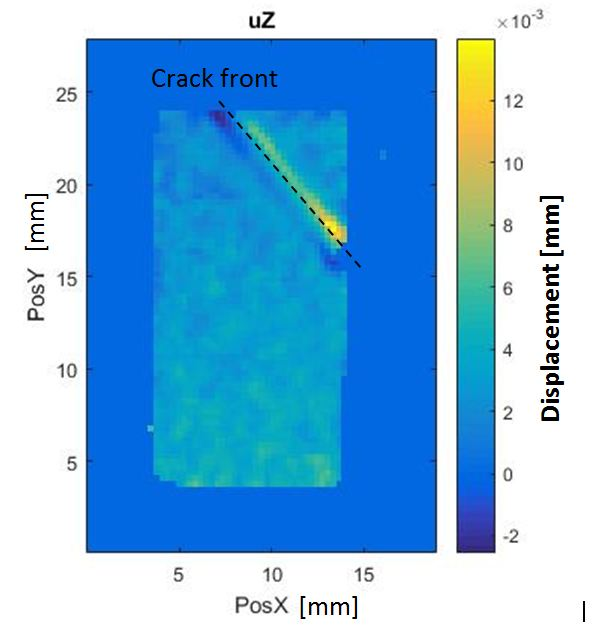
\includegraphics[scale=0.4]{DVC4}
    \caption{Z-direction displacement field on the x-y plane at a height of 15.45 mm in the z direction (DVC)}
    \label{fig:DVC2}
\end{figure}



% The location of this crack front is highlighted in the two images and it can be different at the two different heights 

% DVC displacement fields are very similar to DIC displacement fields in appearance however the difference lies in that DVC computes displacement fields through the thickness of the specimen whereas DIC only presents the displacement data for the specimens surface. 

% allow the user to quickly see what deformation a specimen underwent.

% The x-displacement is almost uniform in the horizontal direction 

% full field
% spatial resolution 
% accuracy
% visulisation 



\chapter{Objectives}
The main aim for this project is to create a unifying program which is capable performing 2D Digital Image Correlation (DIC) or Digital Volume Correlation (DVC) on a given set of images while allowing the user full control over what methods are used to perform each task during the correlation process. The program is to consist of a basic Graphical User Interface (GUI) and a backend which will handle calibration and correlation. The focus of this project is on the backend.

\section{Literature review}
Conduct an in-depth literature review on 2D subset based DIC and DVC. The purpose of this is to obtain a good understanding of the overall calibration and correlation processes involved in gradient-descent, subset based DIC and how these are related to DVC. In doing so special attention will be paid as to how the various DIC algorithms perform the same tasks in the correlation process using different methods. It is these different methods that are to be included in the program as options for how the correlation process can be controlled by the user.

\section{Framework and preliminary backend code}
The next objective is to use the knowledge gained from the literature review to design a framework for how the backend will perform 2D gradient-descent, subset based DIC. This framework will focus on how the different tasks of the correlation process can be separated so that modular code for each method of performing these tasks, identified in the literature review, can be interchanged to perform correlation. This will form the basis of how the user will be capable of controlling how the correlation process is performed.

Once a good framework has been designed the various methods of performing the tasks of the correlation process will be broken down into programmable functions so that a code can be created for each in Matlab. Then these codes will be connected according to the framework to form a first version of the backend of the program for DIC applications.

Thereafter a framework will be designed for DVC which will involve how the DIC framework can be changed to incorporate an extra dimension in the analysis. This framework will then be used to create code for the backend which enables DVC analysis to be performed.

\section{Validating the preliminary backend code}
Once the preliminary backend code has been completed it will be tested to identify bugs and problems. Image sets from previous DIC and DVC experiments will be analysed using this preliminary code to determine displacements. These calculated displacements will be compared to the displacements calculated by the commercial DIC software (LaVison) so that areas of poor correlation can be identified. Simpler experiments such as basic tension tests will be used first so that basic issues and bugs in the code can be identified and fixed. Thereafter more complex experiments such as specimens containing cracks will be used to see what problems arise in the code.

\section{Improve preliminary backend code}
Problems that arise in the preliminary backend code must be fixed. First problems that affect the execution of the code are to be fixed. Thereafter issues specific to material science applications are to be investigated. These are likely to include difficulty in dealing with discontinuous displacement fields, high strain gradients, applied masks and noise robustness. To improve the codes ability with regards to these types of problems additional functions will need to be designed such that they deal with these issues. Once this objective is complete a good backend for 2D DIC and DVC should result.

% \section{Explore new subset matching techniques}
% New and alternative subset matching techniques are to be explored to determine whether they would be beneficial in material science applications.

\section{Creating the GUI}
With the backend functioning properly a framework for communication between the GUI and backend is to be designed. This should be designed in such a way that it will still allow users to communicate directly with the backend without a need for the GUI. Once the framework is finished the backend will be edited to conform to this framework and the GUI layout will be designed according to what codes are available to perform the different correlation tasks and what input parameters are needed for these codes. Thereafter the GUI will be coded in Matlab according to this design.

\section{Validate the program}
Validate the program by quantifying its performance against that of commercial DIC software. In order for the proposed program to be of use it needs to perform at a similar level to that of commercial software. Two types of tests will be used for this. First generated speckle patterns will be deformed according to known displacement fields and the images of these will be correlated using both the proposed and commercial software. The similarity between the calculated displacement fields and the known displacement fields that were applied will give an indication of the performance. 

The second test will involve deforming specimens as images are captured using the commercial DIC system. These images will then be analysed using both the commercial and proposed DIC program. Finally the results of these two will be compared in order to determine whether the proposed program performs to an acceptable level.



% Develop a solid framework and corresponding code which allows full control over a basic 2D DIC algorithm.
% This code should allow full control over what methods are used to complete each aspect of the correlation process and
% the values of parameters that affect how the algorithm is implemented. This is done so that a solid starting point for the
% backend of the software is created.

% Through this the options that affect how the DIC algorithm is implemented, such as the interpolation scheme, can be identified. As the algorithms proposed by various papers are studied; the difference between these modified algorithms and the basic algorithm proposed by Sutton [1] will give an indication of what aspects of the basic algorithm can be performed in different ways. This will help identify what options should be available in the software.

% Key objectives have been identified which if achieved will ensure the main aim is achieved:
% 1. Conduct an in-depth literature review on Digital Image Correlation.
% The purpose of this is to obtain a good understanding of the overall calibration and correlation processes involved in
% gradient descent, subset based DIC. Through this the options that affect how the DIC algorithm is implemented, such as
% the interpolation scheme, can be identified. As the algorithms proposed by various papers are studied; the difference
% between these modified algorithms and the basic algorithm proposed by Sutton [1] will give an indication of what aspects
% of the basic algorithm can be performed in different ways. This will help identify what options should be available in the
% software.

% 2. Develop a solid framework and corresponding code which allows full control over a basic 2D DIC algorithm.
% This code should allow full control over what methods are used to complete each aspect of the correlation process and
% the values of parameters that affect how the algorithm is implemented. This is done so that a solid starting point for the
% backend of the software is created.

% 3. Validate this developed code using experimental data.
% This is done in order to ensure that the code is capable of performing DIC in a real world situation where unexpected
% problems can arise. As a result of attempting to perform DIC on images of actual experiments; the issues in the code and
% areas that need improvement will become apparent.

% 4. Improve the codes ability and robustness for material science applications.
% The issues that arise form the validation tests of objective 3 need to be solved in order for the code to become functional.
% Additional shortfalls specific to material science applications that arise during the test, such as difficulty in dealing with
% discontinuities, high strain gradients, artefacts and noise, are to be investigated in order to develop codes that deal with
% these.

% 5. Extend the code to DVC and develop the GUI.
% Once the 2D DIC code is fully functional it is to be modified to perform DVC. Once this is completed the backend is fully
% operational and the GUI can be designed and programmed so that users can easily control the backend.

% 6. Validate the software by quantifying its performance against that of commercial DIC software.
% In order for the proposed software to be of use it needs to perform at a similar level to that of commercial software. Two
% types of tests will be used for this. First generated speckle patterns will be deformed according to known displacement
% fields and the images of these will be correlated using both the proposed and commercial software. The similarity between
% the calculated displacement fields and the known displacement fields that were applied will give an indication of the
% performance. The second test will involve deforming specimens as images are captured using the commercial DIC
% system. These images will then be analysed using both the commercial and proposed DIC software. Finally the results of
% these two will be compared in order to determine whether the proposed software performs to an acceptable level.

% The overall objective of this project is to create a software package that is capable of performing multiple DIC algorithms on a set of images to determine the deformations that the specimens underwent as the images were taken.

% \begin{itemize}
% 	\item This project will involve the completion of a comprehensive literature review focusing on DIC.
% 	\item A unifying software is to be created which can perform local subset based 2D DIC and DVC on the appropriate images via multiple DIC algorithms. Additionally the user will be able to control how these algorithms are applied to the images. This is to include subset warp function, subset size, step size, interpolation scheme.
% 	\item Research into programming either a FEM based global DIC or using neural networks to solve for underlying displacement fields will be conducted. The purpose of this is to provide an alternative technique which is substantially different from the other algorithms offered so that it can be used in situations where its benefits offer an advantage over the more commonly used subset based methods.
% 	\item The performance of the algorithms contained within the software are to be quantified against the performance of a commercial DIC software (LaVision). The purpose of this is to validate the software to prove it can be reliably used in material science applications.
% \end{itemize}

% \chapter{Objectives}
% Digital Image Correlation is a method that enables the position of an object in an image to be tracked from one image to the next. If the camera remains stationary while images are taken then the difference in position of the object from one image to the next can be used to determine its displacement. Thus images taken of an object in motion can be used to determine the displacement of the object. 

% Over the last 30 years Digital Image Correlation (DIC) has been developing at a steady rate. This, coupled with the increase in resolution of digital cameras and the improved performance of computers according to Moore's law, have made it possible to calculate displacements to a high degree accuracy within a reasonable computation time.

% Furthermore, since only images need to be taken of the object of interest, DIC enables displacement measurement without making contact with the object. This enables DIC to be used in situations where the object is exposed to harsh environments and DIC can still be used to measure displacements.

% As a result DIC has been successfully applied within material science as a method of measuring displacements of test specimens as they are deformed. The use of DIC for material science applications is further beneficial in the fact that only images need to be taken of the specimen in order to determine displacements. Thus DIC is a non-contact method of measuring the displacements. This is advantageous over conventional methods of displacement measurement which need to be in contact with the specimen since being in contact with the specimen can cause the material behaviour to change in certain circumstances. Additionally the specimen can be exposed to harsh environments and a camera can still record images from a safe location such as through a window or behind a shield.

% Furthermore DIC calculates the displacement over the whole surface of the object. That is it calculates the displacement for many points on the surface of the specimen making full-field displacement data available. This is advantageous since it allows more complex material behaviour to be investigated.

% Thus it is clear that DIC holds many benefits for material science applications. Unfortunately commercial DIC software is expensive. DIC systems can cost in excess of R 500 000 putting it out of the reach of many research institutions. Opensource software is available but the validity of the results is not guaranteed.

% However the issue goes beyond this. Software currently available for DIC analysis, commercial or opensource, don't provide the user with sufficient control over the correlation process. The displacements calculated can be heavily dependent on the algorithm used, the convergence criteria selected, the subset size and the allowable subset deformations.

% As a result there are currently multiple algorithms available to (software usually only offer a couple correlation algorithm options)

% commercial expensive
% lack control over algorithm 
% don't know what algorithm is doing- black box
% more uses for DIC
% hold back research
% allows better understanding of material characteristics
% DIC offers a great learning tool for material science
% cameras and computers more powerful and cheaper


% opensource:
% ability for people use it for research purposes
% more publications from SA


% Many papers have shown \todo{add references of papers read} that DIC can be successfully used to measure full field displacements on the surface of objects that are subject to loads. These displacements can then be used to determine the strains and stresses over the surface of objects or through solving an inverse problem the material properties of the object can be determined \todo{reference}. It is clear that this is a powerful tool for material science research.

% However since it is a relatively new and niche technology the software available commercially to perform DIC analysis is expensive and out of reach for many research institutions and business that could otherwise benefit from its use. This is unfortunate since the ever growing capabilities of DIC indicate that is is likely to become an invaluable tool in many material science applications. \todo[inline]{something about how it is a useful tool for teaching which is not possible with how much it costs, how research progress is hindered by lack of access...}

% The aim of this project is to create an open-source DIC program with material science applications in mind so that researchers can make use of it if they do not have access to commercial software. The idea is to offer most of the capabilities of commercial software that is essential for material science applications at a level of accuracy and precision that is comparable to these commercial systems. The purpose is not to replace the commercial systems but to offer an attractive alternative to those who do not have access to them.

% The program is to be separated into a backend which performs the calculations and the frontend which will consist of a Graphical User Interface (GUI) to allow users to control the backend. 
% % Since it is to be open-source the backend is to be written in an freely available programming language (either python of C) so that everyone has access to it. The frontend on the other hand is to be written in Matlab since most research institutions use it for their DIC data analysis. \todo[inline]{might consider a different language once I have tried python out}

% % Many DIC algorithms have been designed over the years, each having characteristic advantages and disadvantages for certain applications. As such the program is to be able to use multiple different correlation algorithms so that the user can choose the one that best suits their specific application. Additionally it is intended that the program be modular with regards to the DIC algorithms so that users can easily write their own algorithms and add them to the programs library.
% \chapter{Objectives}
% \begin{itemize}
% 	\item Completion of this project should result in both a comprehensive literature study on DIC and a DIC program. The program should be capable of taking in images, process these images using on of several available DIC algorithms to determine displacements in the images. The DIC algorithms within the program are to be focused on use in material science applications.
% 	% An in-depth literature review of DIC is to be written and the most promising DIC algorithms for material science purposes are to be identified. These algorithms will include not only subset based DIC but also global DIC. These identified algorithms will then be implemented in the DIC program to be developed.
% 	\begin{itemize}
% 		\item A literature review will be conducted on DIC algorithms both subset based and global DIC.
% 		\begin{itemize}
% 			\item Research will be conducted into DIC and DIC algorithms using articles, research papers and the internet as sources of information. As knowledge is gained it will be added to the literature review.
% 		\end{itemize}
% 		\item The researched DIC algorithms will be sorted into those that would be applicable in material science applications and those that are not.
% 		\begin{itemize}
% 			\item Once the algorithms have been researched they will be identified at beneficial for material science if they have good sub-pixel displacement accuracy, are robust to some degree, have acceptable computational requirements
% 		\end{itemize}
% 		\item Once a DIC algorithm has been identified as beneficial in terms of a material science application it will be coded so that it can be added to the program.
% 		\begin{itemize}
% 			\item Using python as a programming language the identified DIC algorithms will be coded using the research papers and articles as a guide so that they can become a part of the overall program.
% 		\end{itemize}
% 	\end{itemize}
% 	\item One of the main aspects of this project is that the program itself should be opensource so that it is easily accessible. Thus the program is to be separated into a backend which will handle the correlation process and a frontend which will consist of a GUI to give the user an easy method of controlling the backend. The backend is to be programmed in a freely available programming language and it will be capable of being operated without the use of the frontend to ensure that anyone can use it. The frontend will be programmed in Matlab since it is popular amongst research institutions for DIC data analysis.
% 	\begin{itemize}
% 		\item The backend will most likely be written in python since it has great support for scientific computing while being popular. Research into how to program in python is to be conducted in order to be able to write the backend code.
% 		\begin{itemize}
% 			\item Online python learning resources will be used to obtain the basic knowledge of python. More advanced knowledge will be gained during the process of writing the DIC algorithm codes as built in functions are researched on the internet.
% 		\end{itemize}
% 		\item A communication method between the backend and frontend is to be designed such that the backend can be used without the frontend for those who prefer commandline interaction and so users can create their own programs to control the backend. 
% 		\begin{itemize}
% 			\item Research will be conducted on the ways in which programs using different programming languages can communicate with each other so that the method of communication is truly robust. Using a text file as the input to the backend will be used if no better methods are found.
% 		\end{itemize}
% 	\end{itemize}
% 	\item The purpose of the program is to allow the user more control over the correlation process. This includes being able to control the subset size and geometry \todo{not sure about geometry}, the deformations that the subset can undergo, overlapping of the subsets, cost function, convergence criteria, 
% 	\begin{itemize}
% 		\item A framework is to be developed for how the DIC codes are to work in such a way that the above mentioned parameters are controllable across all the algorithms in the same way.
% 		% The code to be written for the various algorithms is to be done in such a way that there exists the same level of control across all the algorithms. This requires modularity within the codes.
% 		\begin{itemize}
% 			\item To design this framework the parameters to be controlled will be identified. Then how these parameters affect each DIC algorithm will be investigated and the DIC codes will be written in such a way that these parameters will be part of the input to the DIC codes so that all the DIC codes communicate with the frontend in the same way with regard to the controllable parameters. As such some of the DIC codes will need to be adjusted so that all the codes are controllable in the same way.
% 		\end{itemize}
% 	\end{itemize}
% 	\item The proposed program will only be of use if its performance is inline with that of commercial software. Thus the program needs to determine displacements to a degree of accuracy and precision that is comparable with that of commercial systems. Computational efficiency and runtime are not a concern in this regard.
% 	\begin{itemize}
% 		\item In order to achieve this objective a method for quantifying the accuracy and precision of DIC algorithms is to be created.
% 		\begin{itemize}
% 			\item Research is to be conducted into the way current DIC system accuracy and precision are quantified using articles, research papers and the internet as resources. With this information a quantification method will be designed. \todo{validating the quantification method?}
% 		\end{itemize}
% 		\item A 2D/3D stereovision camera system is to be designed and assembled for capturing images for DIC.
% 		\begin{itemize}
% 			\item Either buying another of the cameras already available in the research group (Rollans skripise) or researching appropriate cameras and purchasing the best option. Once cameras have been acquired a data acquisition system is to be obtained to capture the images simultaneously on both cameras at the same time. \todo{sync with commercial system so all images are simultaneous}
% 		\end{itemize}
% 		\item Two experiments are to be designed. One will be a synthetic test that will provide the DIC programs (commercial and proposed) with generated images of known displacements and the algorithms will be assessed in terms of how close their calculated displacements are to the actual values. 
% 		\begin{itemize}
% 			\item A good speckle pattern will be generated and then displacements will be applied to this speckle pattern so that deformed images are obtained. A variety of deformations will be used so that the limits of the algorithms can be identified. This will likely include rotations so that the algorithms can be evaluated in terms of their ability to track rotation.
% 			\item The image sets will be processed by all the DIC codes and the resulting displacement data will be compared to that of the known displacements to give an indication of the level of performance of the algorithms for synthetic data.
% 			\item Ideally the quantification method will be used to provide meaningful information on the performance of the codes.
% 			\item Problems identified with the codes, in doing these tests, will be fixed so that they perform as best as possible in the next test. 
% 		\end{itemize}
% 		\item The second experiment will test the algorithms in a real world situation. The Stellenbosch commercial DIC camera system and a self designed system will be used to capture images of the same specimens being deformed. These images will then be processed through the respective systems (commercial DIC and opensource) in order to compare their performance in a real world situation.
% 		\begin{itemize}
% 			\item A couple specimens will be designed and manufactured. The specimens are to be designed in such a way that some deform in a way that is beneficial for DIC purposes and some will be designed to deform in a way that is detrimental for DIC. This will give a good overall indication of the capabilities of the codes.
% 			\item Specimens will be deformed as images are taken of them by the commercial DIC camera system and the in house camera system; preferably these systems will be set to capture images simultaneously so that the images of both the commercial and inhouse systems are of the specimen under the same deformation.
% 			\item These images will be masked and processed by the commercial and proposed DIC codes to obtain displacement data. This data will be analysed using the quantification method mentioned above so that the proposed DIC codes can be compared to that of the commercial system and to each other.
% 		\end{itemize}
% 	\end{itemize}
% \end{itemize}

% \begin{itemize}
% 	\item An in-depth literature review is to be conducted into DIC so that the main DIC algorithms for material science purposes can be identified and a deep understanding of the overall DIC process can be obtained.
% 	\item The program should be a good alternative to commercial programs for material science applications with regards to both 2D and 3D stereo-vision DIC. For this to be a reality the program must have a similar performance level to that of commercial software in terms of accuracy and precision of the full field displacements.
% 	\item Multiple DIC algorithms are available with different advantages and disadvantages. As such the program is to offer the user a choice of algorithms so that they can choose the one that suits their situation best. Thus the idea is to allow the user to have more control over the correlation process.
% 	\item In addition to multiple algorithms being available for use; these algorithms are to be implemented in a modular way so that the user can easily create their own algorithms and add it to the programs library. \todo[inline]{not sure if this is possible yet}
% 	\item Since the idea is to offer a good alternative to commercial software; the programs backend (which handles the calculations) is to be written in a freely available language such as python or C. The front end (the GUI) is to be written in Matlab since this is what most research institutions use to analyse DIC data.
% 	\item An image capturing system is also to be designed so that the open-source program can be compared to the commercial software over the whole DIC process from image capturing until the calculation of displacement data. This image capturing system is to be capable of both 2D (one camera) and 3D stero-vision (two cameras) DIC.
% 	\item A bonus objective would be to design the code to execute in an efficient manner so that it completes the correlation process in the shortest time possible. Additionally it would be ideal to structure program in such a way that parallel processing is possible so that further reduction in runtime is possible.
% \end{itemize}
% \section{Research design}

\chapter{Scope}
This project is limited to the aspects listed below. Note that the proposed program is not intended to capture images or perform 3D DIC.
\begin{itemize}
	\item Developing the backend of the program such that it is capable of performing 2D gradient descent, subset based DIC and DVC on a given set of images to output the displacements present in the images. The backend is to allow the user to select what methods are used during the correlation process.
	\item Developing a GUI for the program that allows the user import images, set up the type of analysis, set up the configuration for the correlation process, tell the backend to perform the correlation process and display the results.
	\item Testing the proposed program in order to validate it. The program will be tested using synthetic and real world data to determine how well it performs.
	\item Design specimens for the experiments that are to be performed to validate the program.
\end{itemize}

\chapter{Research planning}
The research plan consists of activities that are closely based on the objectives of the project. The activities are first described and then the time frame, requirements, outputs, cost and milestones of the activity are given.

\section{Literature review}
An in-depth literature review on 2D gradient descent, subset based DIC and DVC are to be conducted in order to develop a good understanding of how these methods work and what steps are involved in the calibration and correlation processes. DIC will be investigated first since it is the simplest type of DIC and so will be easiest in terms of learning the basic concepts. Once a good understanding of DIC is acquired research will move to DVC which is closely related to 2D DIC.

As the different proposed 2D DIC algorithms are investigated special attention will be paid to the ways in which these algorithms use different methods to perform the necessary correlation tasks. Thus as the literature review is conducted a map of how the correlation process works and what tasks need to be completed during its execution will be developed. Then when the different algorithms are investigated their methods of performing these tasks will be documented and a list of the possible ways of performing each task of the correlation process will be created.

\paragraph{Time frame}
01/06/2017 - 30/08/2017

\paragraph{Requirements}
Literature material is necessary for this step. The majority of this material is easily accessible using the internet and other material can be obtained through the Stellenbosch library.

\paragraph{Outputs}
Good understanding of how 2D DIC and DVC work. A map of how the correlation process works and a list of the different methods that can be used to perform the various correlation steps.

\paragraph{Cost} 
No cost is expected to be incurred during this activity.

\paragraph{Milestones}
Gain sufficient understanding in order to start developing a framework for DIC and DVC.

% \ganttbar{\small Literature review}{2017-06-01}{2017-09-30}\\
% \ganttbar{\small DIC framework}{2017-08-02}{2017-10-10}\\
% \ganttbar{\small Program the backend}{2017-10-11}{2017-11-30}\\
% \ganttbar{\small Test the backend}{2017-12-01}{2017-12-30}\\
% \ganttbar{\small Specimen design}{2018-01-01}{2018-01-08}\\
% \ganttbar{\small Improve backend}{2018-01-09}{2018-02-28}\\
% \ganttbar{\small Create DVC code}{2018-03-01}{2018-03-31}\\
% \ganttbar{\small Create GUI}{2018-04-01}{2018-04-16}\\
% \ganttbar{\small Validate the software}{2018-04-17}{2018-05-15}\\
% \ganttbar{\small Write up thesis}{2018-05-16}{2018-08-01}\\

\section{DIC framework}
The map of the correlation tasks and the list of the different methods of performing these tasks will be used to create a framework for the DIC part of the backend of the program. First the tasks that need to be performed during correlation, the order in which these tasks need to be performed, the methods that can be used to perform these tasks and what information transfer each of these methods involve will be used to create a detailed structure of how the tasks can be arranged and connected in such a way that these different methods of performing the tasks can be used interchangeably.

Thereafter each method of performing the correlation tasks will be analysed and broken down into programmable functions. The connection and communication between these functions will then be used to create a map for each method. The detailed structure of the correlation tasks and these maps for all the methods will then be combined to create a framework for the overall backend of the program. 

This framework will then be used as a basis to develop a similar DVC framework. These frameworks will be similar to one another with the DVC framework basically including an extra dimension to be analysed. These two frameworks will then be combined to give the overall backend framework.

The purpose of this backend framework is to break down the overall correlation problem into the straight forward functions that need to be performed. These straightforward functions are then relatively easy to program and connect together to form the backend of the program.

\paragraph{Time frame}
01/09/2017 - 10/10/2017

\paragraph{Requirements}
The map of how the correlation process works and a list of the different methods that can be used to perform the various correlation steps are needed in order to develop the framework.

\paragraph{Outputs}
A comprehensive framework for 2D DIC and DVC that allows user control over options for the correlation process.

\paragraph{Cost} 
No cost is expected to be incurred during this activity.

\paragraph{Milestones}
Complete framework for backend.

\section{Program the backend}
In this activity the functions identified in the backend framework are to be written into code. Then once code exist for all these functions the codes will be connected according to the framework to create the backend of the program. This backend is to be capable of both 2D DIC and DVC analysis.

As the codes are being developed they will be tested by using synthetic tests. In these tests an image of a generated speckle pattern will be deformed according to a chosen displacement function to produce a deformed image. Then these images will be analysed using the backend and the difference between the calculated displacements will serve as a means of identifying faulty code and bugs. These issues will be fixed as they are identified.

Matlab is to be used as the programming language since most research institutions use it to analyse DIC data. Thus it is reasoned that anyone who want to use DIC software which allows this level of control over the correlation algorithm is likely to have access to Matlab.

\paragraph{Time frame}
11/10/2017 - 30/11/2017

\paragraph{Requirements}
The framework for the backend is needed as an input for this activity. Additionally Matlab and a computer are required for programming purposes.

\paragraph{Outputs}
A working backend for the program coded in Matlab.

\paragraph{Cost} 
Since Matlab and a computer are provided by the university no cost are anticipated.

\paragraph{Milestones}
Create a working backend code to perform 2D DIC and DVC analysis.

\section{Validate the backend}
Once the backend is finished it will be tested on actual DIC and DVC image sets from material science experiments. The purpose of this is to identify any fundamental issues in the backend and to identify issues specific to material science applications. A list of the issues is to be created so that they can be improved on. Issues will be identified by areas of poor correlation and discrepancies between the results of the proposed program and that of the commercial software (LaVision).

Various types of material science experiments will be used in order to identify as many material science related issues as possible. Anticipated issues include difficulty in dealing with displacement discontinuities, applied masks, high strain gradients and noise.

Various correlation process configurations of the different methods of performing the correlation tasks will be used in order to identify which methods have the greatest impact on the results and to identify issues that arise with using certain methods.

\paragraph{Time frame}
01/12/2017 - 30/12/2017

\paragraph{Requirements}
A working backend which is created in the previous activity. Commercial DIC software which is available at Stellenbosch University. Matlab and a computer which has been provided by Stellenbosch University. Material science experiment image sets, to be analysed, which are already available on the DIC computer of the material science research group. 

\paragraph{Outputs}
A list of issues to be fixed in the backend. These issues include problems specific to material science applications. Additionally an understanding of what types of displacement fields cause the biggest issues for the backend.

\paragraph{Cost} 
All of the required equipment is already available at Stellenbosch University and so this activity is not expected to any costs.

\paragraph{Milestones}
Identify issues that need to be fixed or improved within the backend code.

\section{Specimen design}
The specimens required for validating the program are to be designed and manufactured. This is done at this stage in the project in order to allow ample time for the specimens to be manufactured so that no delays occur later in the project when time restrictions are strict. Additionally after completing the testing of the algorithms in the previous activity the displacement fields that are unfavourable for the DIC code will become apparent. The specimens can then be designed in such a way that they will produce similar displacement fields so that the DIC algorithms can be put to the test.

All the specimens are to be designed such that they are loaded in tension. The standard dog-bone tension specimen is to be used as a starting point for the specimens and its geometry will be modified in order to create interesting displacement fields. An example of this would be a dog-bone specimen with a hole in the middle. FEM will be used to ensure that the proposed specimen designs will result in the desired displacement fields.

\paragraph{Time frame}
01/01/2018 - 08/01/2018

\paragraph{Requirements}
Material for the specimens. Knowledge of what displacement fields are unfavourable for the backend (obtained from previous activity). CAD software for designing the specimens which is provided by Stellenbosch University. FEM software for developing the specimen designs is provided for by Stellenbosch University.

\paragraph{Outputs}
The specimens to be tested later on in the project to validate the program.

\paragraph{Cost} 
The cost of the materials and the cost of the manufacturing the specimens. - R2000

\paragraph{Milestones}
Creation of specimen designs for manufacturing.

\section{Improve backend}
The issues identified in the backend are to now be solved. Fundamental issues will be solved first since they are specific to the codes already developed for the backend. Thereafter methods of solving issues specific to material science applications will be investigated.

Once methods have been developed to improve the performance of the code in material science applications it will be tested by using the experimental image sets used to first identify issues. The the previous results will be compared to the new results to determine whether there has been an improvement.

\paragraph{Time frame}
09/01/2018 - 14/03/2018

\paragraph{Requirements}
A list of issues that have been identified in the backend.

\paragraph{Outputs}
A more robust backend code that is less susceptible to errors when being used for material science applications.

\paragraph{Cost} 
This activity involves no cost.

\paragraph{Milestones}
Produce a backend capable of performing 2D DIC and DVC analysis for material science applications.

\section{Create the GUI}
A GUI is to be created to allow the user to easily control the backend without the need to use command prompt. Before work on the GUI is started a method of communication between the GUI and backend is to be designed. This method of communication should be flexible so that the user can still make use of the backend without the GUI if they so desire. With this method of communication finalised the backend is to be refined to conform to this communication method. This will likely only involve minor changes.

Once a method of communication has been developed the GUI can be designed. The GUI layout will be designed according to the structure of the backend. That is the GUI layout is to be arranged such that the different options available for the correlation process are presented in a logical way. Once a layout has been decided upon the GUI will be programmed in Matlab. Matlab's GUI environment offers sufficient GUI elements for the creation of a GUI of this type. Finally the GUI will be connected to the backend. At this point the proposed program should be fully operational.

\paragraph{Time frame}
15/03/2018 - 15/04/2018

\paragraph{Requirements}
Fully functioning backend. A list of the correlation options to be provided; which will be included in the framework developed for the backend.

\paragraph{Outputs}
A GUI and a refined version of the backend which together form the proposed program.

\paragraph{Cost} 
No cost is expected to be incurred during this activity.

\paragraph{Milestones}
Create the final working version of the program (GUI and backend).

\section{Validate the program}
The proposed program is to be validated by comparing its performance to that of commercial software (LaVision) in two types of tests. The first test is a synthetic test similar to that used during the backend's development to check that the code operates correctly. However this time the calculated displacement fields of the various algorithms will be compared to the actual applied displacement field with the difference between the two giving an indication of the accuracy of the algorithm. 

Different applied displacement fields will be used in order to identify shortcomings in the developed algorithms. This will be done by using some displacement fields which are not favourable for DIC and DVC such as those containing significant rotation, displacement discontinuities and large straining. These shortcomings are important since commercial software usually includes ways of dealing with these difficulties. Thus comparing the performance between the commercial software and
proposed program in this regard is important.

Additionally in order to evaluate how well these algorithms deal with noise a second version of the synthetic test will be conducted. In this second version noise will be added to the deformed image that is to be generated and the deviation of the results from the noise free case will be used to indicate sensitivity to noise.

The second test is more representative of real world use of the program. For this test a speckle pattern is applied to each of the aforementioned specimens before securing them in a tensile testing rig. Then images are taken of the speckle pattern using the available commercial system (LaVision) as the specimen is loaded in tension. These images are then analysed using the commercial software and the proposed program in order to determine the underlying displacement fields. 

The same images will be used for all the algorithms so that they can be compared solely on their correlation performance. The commercial system is used to capture images in order to give the commercial DIC software its best use case so that its results can be treated as the golden standard by which the proposed algorithms are compared. 

Once these tests have been conducted the results will be used to decide whether the proposed algorithms perform acceptably well compared to the commercial software. Note that the results of the second test will be relative to the commercial software and not an absolute indication of performance.

\paragraph{Time frame}
16/04/2018 - 15/05/2018

\paragraph{Requirements}
Fully functioning version of the proposed program as created in the previous activity. Matlab, a computer and the commercial DIC software (LaVision) which are all available at Stellenbosch University. The specimens which have been designed and manufactured. A tensile test rig and a commercial DIC camera system which are already available at Stellenbosch University. Spray paint for applying speckle patterns to the specimens.

\paragraph{Outputs}
Data indicating the performance of the propose program and the commercial DIC software (LaVision) for the same tests.

\paragraph{Cost} 
Spray paint - R200

\paragraph{Milestones}
Obtain data on the performance of the proposed program.

\section{Write up thesis}
In this activity the information gained throughout this project is to be organised and broken down so that it can be reported on in the thesis. 

\paragraph{Time frame}
16/05/2018 - 01/08/2018

\paragraph{Requirements}
Literature review must be conducted prior to this. Results indicating the performance of the proposed program. Latex to write the report.

\paragraph{Outputs}
A report summarising the important aspects of the project.

\paragraph{Cost} 
Since latex is free no costs will result.

\paragraph{Milestones}
Complete the report.

% First an in-depth literature review is to be conducted in order to obtain a deep understanding of the Digital Image Correlation process and to identify algorithms that are important for use in material science. Once the core algorithms have been identified codes will be written for them in such a way that these algorithms communicate with the main backend in a similar way. This will allow the algorithms to be modular so that the user can easily select which one they would rather use. Additionally these codes must allow the user to control parameters within each of the chosen core algorithms so that the user can have a large degree of control over the correlation process.

% Once this is completed the main backend program will be developed in such a way that it is capable of communicating with the fontend that is to be designed. A method of using commands in a text file is likely to be the best method of choice so that the user can also control the backend directly if they so desire. Hereafter the frontend GUI is to be designed and coded.

% Once the software is working properly testing can start to identify problems and areas that need improvement. In order to validate the program a test needs to be devised that evaluates the accuracy and precision of the program compared to that of the commercial software. This is likely to cover such issues as sensitivity to rotation and rigid body motion, how the program performs in calculating displacements near regions of discontinuity on the surface of the specimen (such as near cracks) and performance on the edge of the specimen. Additional concerns with regards to performance will be identified when conducting the literature review.

% Initial testing will be done based on images generated with known displacements so that it is only the software's performance that is being analysed. After testing of this type has identified problems and these problems have been fixed; testing the program on actual images of loaded specimens can be conducted. For this testing to be possible it is necessary to design an image capturing system so that images can be taken of the specimen that is deforming. Ideally the software side of this system will form part of the main program.

% For this type of testing specimens should be designed so that they exhibit displacements that are both favourable and detrimental to DIC so that the overall performance of the program in multiple situations can be determined. It is these results that will indicate whether the program is successful in its objective of being comparable in terms of accuracy and precision with commercial software.

% Once the program is performing as desired it can be re-evaluated to see whether it could be implemented in a more efficient manner or if it could be implemented in such a way that parallel processing is possible so that it takes less time to complete a correlation process.

% \chapter{Resources required}
% The following resources are required in order to complete this project.
% \begin{itemize}
% 	\item A tensile testing rig is required in order to complete the second validation test. An MTS tensile test rig is available in the Stellenbosch labs which is fully capable of performing the proposed tests. Additionally the necessary clamps for tension specimens are also available.
% 	\item Specimens must be designed and manufactured. The specimens are to be designed on CAD software which is available at Stellenbosch University. The specimens can then be manufactured either in the Stellenbosch Mechanical Engineering workshop or specimen manufacturing can be outsourced to an appropriate supplier. The choice of which manufacturer will be based on material choice and required tolerances. FEM software used for designing the specimens is also available from Stellenbosch University. The materials for the specimens will be provided by the chosen manufacturer.
% 	\item Matlab and a computer is necessary for programming the software. Matlab is available at Stellenbosch University and a computer has been provided by Stellenbosch University.
% 	\item A commercial DIC system is necessary for the validation tests and for conducting the experiments on the designed specimens. A LaVision commercial DIC system (camera and software) is available from Stellenbosch University.
% 	\item Spray paint is needed in order to apply the speckle patterns to the specimens. This paint will be purchased when it is needed.
% 	\item Literature resources are required for the literature review. The Stellenbosch University library provides access to most literature resources that will be needed.
% 	\item Latex is to be used to write the thesis report. This software is freely available for use.
% 	\item Experimental data is required for testing the backend to find issues. Old experimental data is available from the Materials Engineering research group at Stellenbosch University.
% \end{itemize}

\chapter{Budget}
The table below provides an outline of the expected costs for this project organised according to the activities in which the expenses are expected to occur. Since most of the resources required for the completion of this project are already available from Stellenbosch University the overall cost of the project is rather low.
\begin{center}
\begin{tabular}{|c|c|c|}
\hline
 Activity & Resource & Cost \\ 
 \hline
 \hline
 Literature review & Internet and research papers & 0 \\
 \hline
 DIC framework & NA & 0\\
 \hline
 Program backend & Matlab & 0\\
 \hline
 Validate the backend & Commercial software & 0\\
  & Matlab & 0\\
  \hline
 Specimen design & Materials and manufacturing & 2000\\
 & CAD software & 0\\
 & FEM software & 0\\
 \hline
 Improve backend & Matlab & 0\\
 \hline
 Create GUI & Matlab & 0\\
 \hline
 Validate program & Tensile testing rig & 0\\
 & Commercial DIC system & 0\\
 & Spray paint & 200\\
 \hline
 Write up thesis & Latex & 0\\
 % Matlab & Software necessary for programming & - \\  
 % \hline
 % Specimens & Cost of manufacturing the specimens necessary to validate the software & 2000 \\
 % \hline
 % DIC system & Cost of using the DIC system for validation tests & - \\
 % \hline
 % Tensile tester & Cost of using the tensile testing machine for the validation tests & - \\
 % \hline
 % Spray paint & Paint needed to apply the speckle patterns to the specimens & 200 \\
 \hline
 Total & & 2200 \\
 \hline
\end{tabular}
\end{center}




\begin{landscape}
\chapter{Time-frame}
\begin{figure}[htbp!]
\begin{center}

% \begin{ganttchart}[y unit title=0.4cm,
% y unit chart=0.5cm,
% vgrid,hgrid, 
% title label anchor/.style={below=-1.6ex},
% title left shift=.05,
% title right shift=-.05,
% title height=1,
% bar/.style={fill=gray!50},
% incomplete/.style={fill=white},
% progress label text={},
% bar height=0.7,
% group right shift=0,
% group top shift=.6,
% group height=.3,
% group peaks={}{}{.2}]{24}
% \begin{ganttchart}[y unit title=0.4cm,
% y unit chart=0.5cm,
% vgrid,hgrid, 
% title label anchor/.style={below=-1.6ex},
% title left shift=.05,
% title right shift=-.05,
% title height=1,
% bar/.style={fill=gray!50},
% incomplete/.style={fill=white},
% progress label text={},
% bar height=0.7,
% group right shift=0,
% group top shift=.6,
% group height=.3,
% ]{24}
\begin{ganttchart}[hgrid,y unit title=0.4cm,y unit chart=0.4cm,time slot format=isodate,
link bulge=6,x unit=0.3mm,
milestone/.append style={xscale=0.3cm},
milestone/.append style={fill=orange},
bar/.append style={fill=yellow},
link/.append style={color=blue}]{2017-06-01}{2018-09-30} %link label anchor/.style=below,
%labels
\gantttitlecalendar{year, month} \\
\ganttbar{\small Literature review}{2017-06-01}{2017-08-30}\\
\ganttmilestone{\small Understanding for framework}{2017-08-30}\\
\ganttbar{\small DIC framework}{2017-09-01}{2017-10-10}\\
\ganttmilestone{\small Comprehensive framework}{2017-10-10}\\
\ganttbar{\small Program the backend}{2017-10-11}{2017-11-30}\\
\ganttmilestone{\small Preliminary backend}{2017-11-30}\\
\ganttbar{\small validate the backend}{2017-12-01}{2017-12-30}\\
\ganttmilestone{\small Identify issues}{2017-12-30}\\
\ganttbar{\small Specimen design}{2018-01-01}{2018-01-08}\\
\ganttmilestone{\small Specimen designs}{2018-01-08}\\
\ganttbar{\small Improve backend}{2018-01-09}{2018-03-14}\\
\ganttmilestone{\small Functioning backend}{2018-03-14}\\
% \ganttbar{\small Create DVC code}{2018-03-}{2018-03-31}\\
\ganttbar{\small Create GUI}{2018-03-15}{2018-04-15}\\
\ganttmilestone{\small Final program}{2018-04-15}\\
\ganttbar{\small Validate the program}{2018-04-16}{2018-05-15}\\
\ganttmilestone{\small Program performance}{2018-05-15}\\
\ganttbar{\small Write up thesis}{2018-05-16}{2018-08-01}\\
\ganttmilestone{\small Thesis report}{2018-08-01}\\
\ganttlink{elem0}{elem1}
\ganttlink{elem1}{elem2}
\ganttlink{elem2}{elem3}
\ganttlink{elem3}{elem4}
\ganttlink{elem4}{elem5}
\ganttlink{elem5}{elem6}
\ganttlink{elem6}{elem7}
\ganttlink{elem7}{elem8}
\ganttlink{elem8}{elem9}
\ganttlink[link type=rdldr*, link bulge 2=18, link mid=0.168]{elem7}{elem10}
\ganttlink[link type=rdldr*, link bulge 2=120, link mid=0.1]{elem9}{elem14}
\ganttlink{elem10}{elem11}
\ganttlink{elem11}{elem12}
\ganttlink{elem12}{elem13}
\ganttlink{elem13}{elem14}
\ganttlink{elem14}{elem15}
\ganttlink{elem15}{elem16}
\ganttlink{elem16}{elem17}
% \ganttlink{elem1}{elem2}
% \ganttlink[link type=s-s]{elem0}{elem2} 
% % \ganttlink[link type=f-s]{elem1}{elem2}
% % \ganttlink[link type=f-s]{elem2}{elem3}
% \ganttlink[link type=f-s]{elem3}{elem4}
% % \ganttlink[link type=f-s]{elem4}{elem8}
% \ganttlink[link type=f-s]{elem3}{elem5}
% \ganttlink[link type=f-s]{elem5}{elem6}
% \ganttlink[link type=f-s]{elem6}{elem7}
% \ganttlink[link type=f-s]{elem7}{elem8}
% \ganttlink[link type=f-s]{elem3}{elem5}
% \ganttlink[link type=f-s]{elem5}{elem6}
% \ganttlink[link type=f-s]{elem6}{elem7}
% \ganttlink[link type=f-s]{elem7}{elem8}
% \ganttlink[link type=f-s]{elem8}{elem9}


% \gantttitlecalendar{year, month} \\
% \ganttbar{\small Literature review}{2017-06-01}{2017-09-30}\\
% \ganttmilestone{\small Understanding for framework}{2017-08-01}\\
% \ganttbar{\small DIC framework}{2017-08-02}{2017-10-10}\\
% \ganttbar{\small Program the backend}{2017-10-11}{2017-11-30}\\
% \ganttbar{\small Test the backend}{2017-12-01}{2017-12-30}\\
% \ganttbar{\small Specimen design}{2018-01-01}{2018-01-08}\\
% \ganttbar{\small Improve backend}{2018-01-09}{2018-03-14}\\
% % \ganttbar{\small Create DVC code}{2018-03-}{2018-03-31}\\
% \ganttbar{\small Create GUI}{2018-03-15}{2018-04-15}\\
% \ganttbar{\small Validate the program}{2018-04-16}{2018-05-15}\\
% \ganttbar{\small Write up thesis}{2018-05-16}{2018-08-01}\\
% \ganttlink[link type=s-s]{elem0}{elem2} 
% % \ganttlink[link type=f-s]{elem1}{elem2}
% % \ganttlink[link type=f-s]{elem2}{elem3}
% \ganttlink[link type=f-s]{elem3}{elem4}
% % \ganttlink[link type=f-s]{elem4}{elem8}
% \ganttlink[link type=f-s]{elem3}{elem5}
% \ganttlink[link type=f-s]{elem5}{elem6}
% \ganttlink[link type=f-s]{elem6}{elem7}
% \ganttlink[link type=f-s]{elem7}{elem8}
\end{ganttchart}
\end{center}
\caption{Gantt chart}
\end{figure}
\end{landscape}
\chapter{Conclusion}
This document proposes a research project aimed at creating a program for Matlab that is capable of performing DIC or DVC on a given set of images. The proposed program is aimed at providing the user with full control over the correlation process so that users no longer need to treat DIC and DVC as a black box. This project is not intended to have any direct application in industry but rather to provide researchers with a comprehensive tool to perform correlation to determine material deformation.

The motivation of the project has been outlined along with literature review on DIC. The objectives of the project have also been outlined with a research plan which is aimed at achieving these objectives. A time-line for the activities of the research plan is also provided. It is evident that sufficient knowledge and resources are available for the successful completion of this project.
% \section{Outline of chapters}
\bibliography{references}
\bibliographystyle{plain}
\end{document}




% website for computer vision http://dblp.uni-trier.de/db/journals/ivc/ivc29.html


% Are you a vault dweller, cause you seem pretty S.P.E.C.I.A.L. to me





% https://drive.google.com/uc?export=download&confirm=TXgS&id=0B8ChoAcEOa4HbWxmbGFPV2M0aHM
% https://drive.google.com/uc?export=download&confirm=3xOY&id=0B8ChoAcEOa4HaEljZllabTZaeEk
% https://drive.google.com/uc?export=download&confirm=Lu4C&id=0B8ChoAcEOa4HcHZJMlZLeHdwdnc
% https://drive.google.com/uc?export=download&confirm=Qic1&id=0B2LiEl8up6X_R1V5NkF2NVhwaG8
% https://drive.google.com/uc?export=download&confirm=Qic1&id=0B2LiEl8up6X_R1V5NkF2NVhwaG8
% https://drive.google.com/uc?export=download&confirm=78XC&id=0B_q296AKMRsBUGtORW1jQ0lKQzQ


% https://drive.google.com/uc?export=download&confirm=cxmO&id=0B56v3YurenhzYTRXZGZ6MzJOWnc